\newpage
\section{Technical Specifications}

\subsection{Cable Jacket}

  Due to the geographical location of the telescope and weather conditions, it was decided to install a military-grade type of cable for the telescope protecting from any adverse conditions or hazardous environment. 

\begin{figure}
  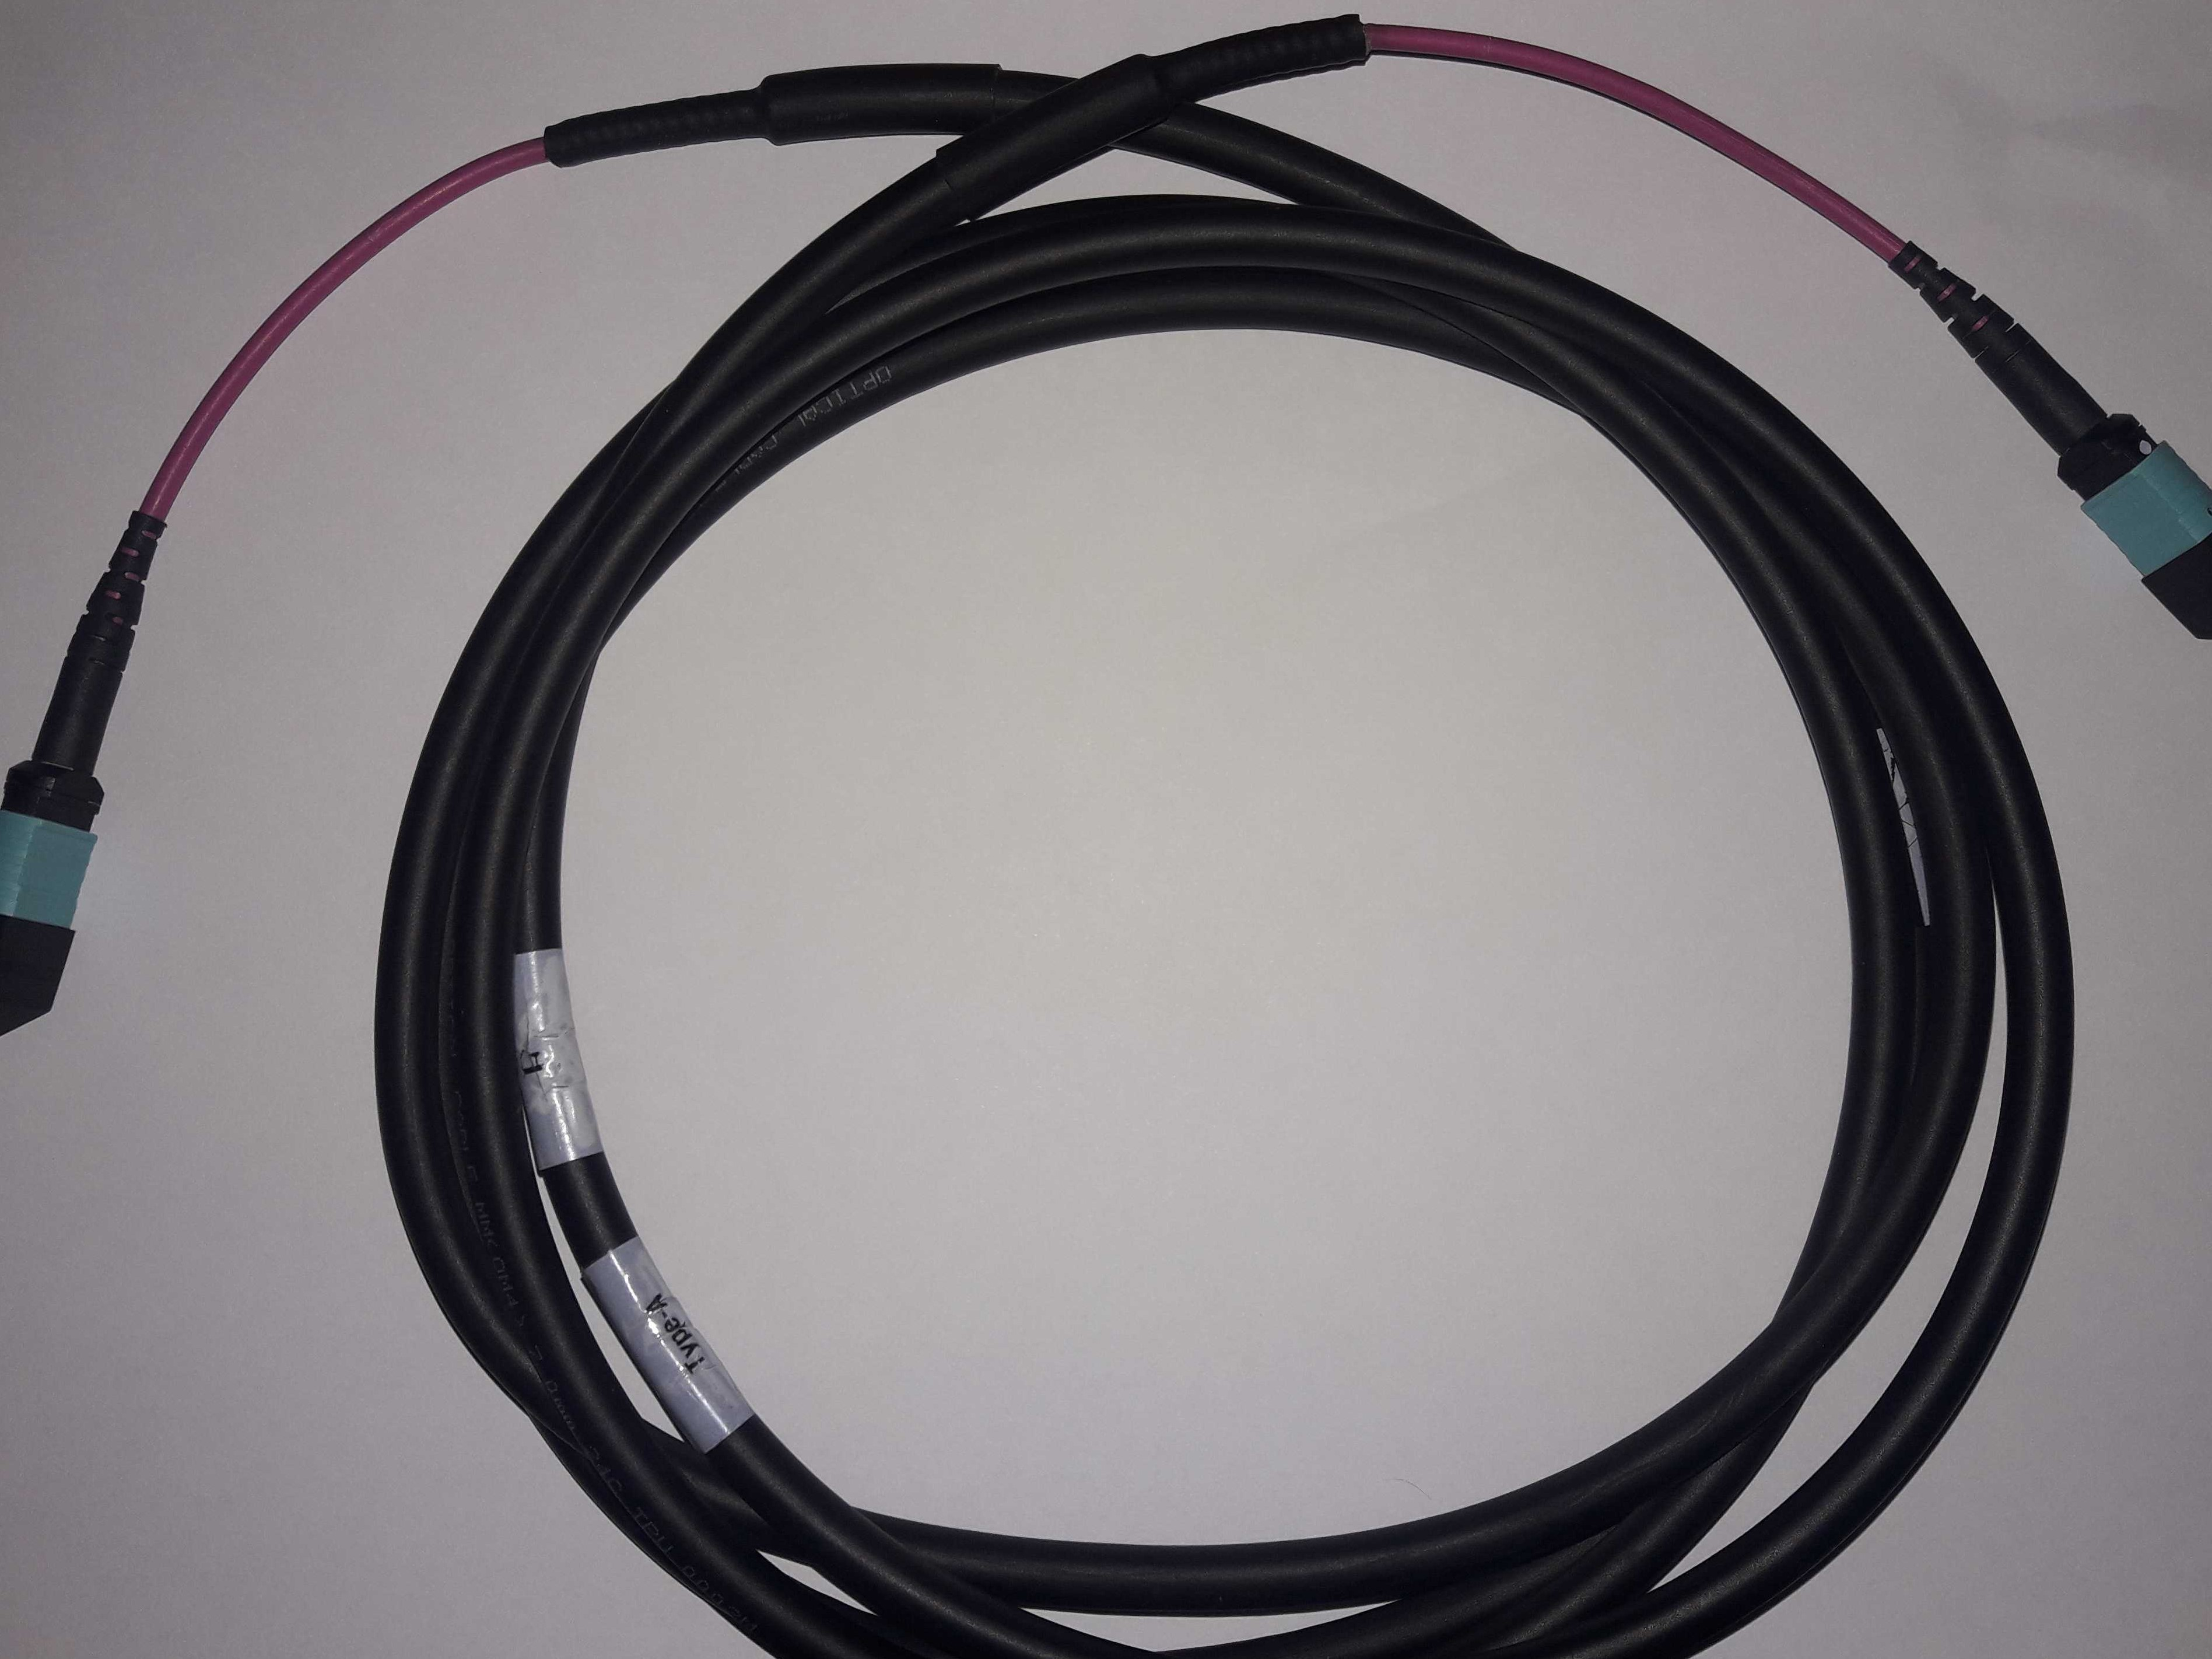
\includegraphics[width=11cm]{images/mtp_militar_cable.jpg}
  \centering
  \caption{Prototype of the Armored Cable}
\end{figure}

This Armored Tactical Cable has the following features:

\begin{itemize}
  \item Strong tensile strength.
  \item Strong resistance to pressure.
  \item Flexible and resistant to any type of bending.
  \item Resistant to oil, wear, and fire.
\end{itemize}

\newpage
Additional Technical Specifications:

\begin{figure}
  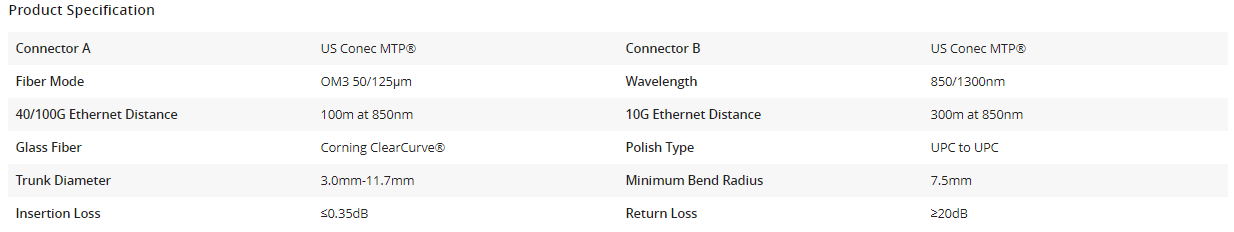
\includegraphics[width=\textwidth]{images/2.png}
  \caption{MTP/MPO Connectors}
\end{figure}


\newpage
\subsection{MTP / MPO connectors and adapters}

  MTP/MPO main characteristics and features

\subsubsection{MTP/MPO Connector}

  Each cable contains 24 filaments with 1 MTP/MPO connector at each end.

\begin{figure}
  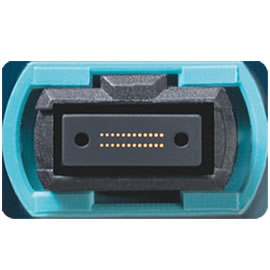
\includegraphics[width=5cm]{images/3.jpg}
  \centering
  \caption{MTP/MPO Connectors}
\end{figure}

\newpage
\subsubsection{MTP/MPO Adapters}

  Each connection between cables has to use a key-up and key-down adapter in order to work and function properly.

\begin{figure}
  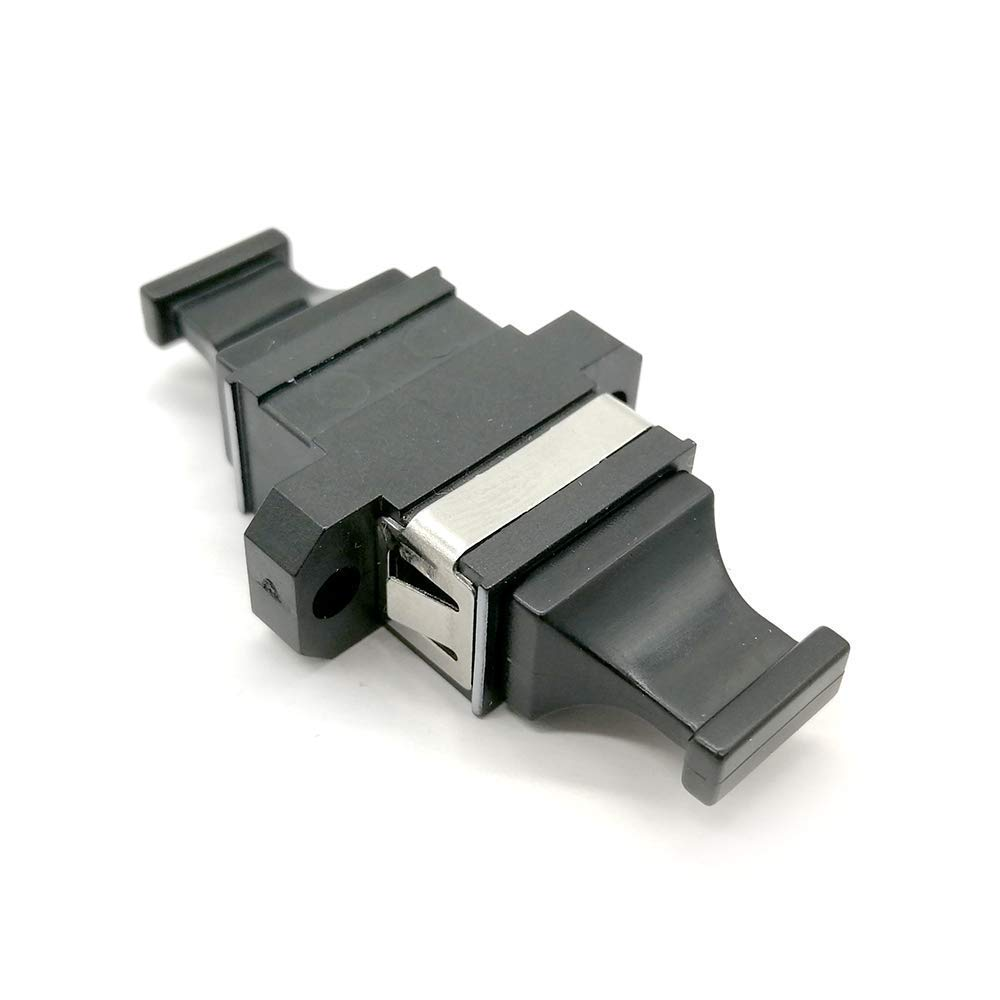
\includegraphics[width=6cm]{images/4.jpg}
  \centering
  \caption{Key-up and Key-down adapter}
\end{figure}

\newpage
\subsubsection{The MTP / MPO Female and Male Connectors}

  The MTP/MPO cables always connect to another MTP/MPO cable, each connector has a connection type which is either Female or Male.

\begin{figure}
  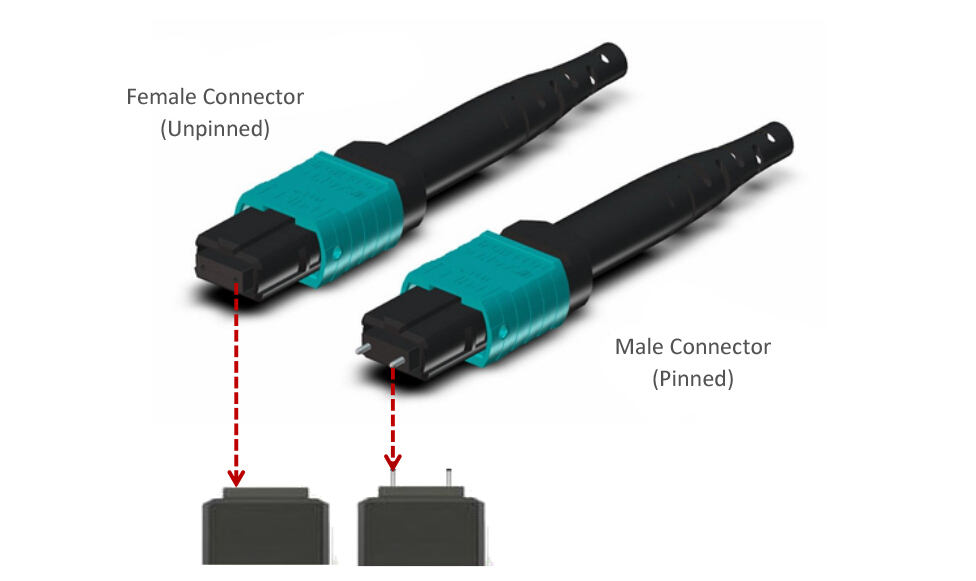
\includegraphics[width=\textwidth]{images/5.jpeg}
  \caption{MTP/MPO Connectors Female/Male}
\end{figure}

\newpage 
\subsubsection{Cable Polarity}

  The cable can be purchased in 3 polarity modes, these are:

      Type A
      Type B
      Type C

  For documentation purposes, we will turn our focus on Polarity Type-A cables.

\begin{figure}
  \centering
  \begin{subfigure}{0.48\textwidth}
    \centering
    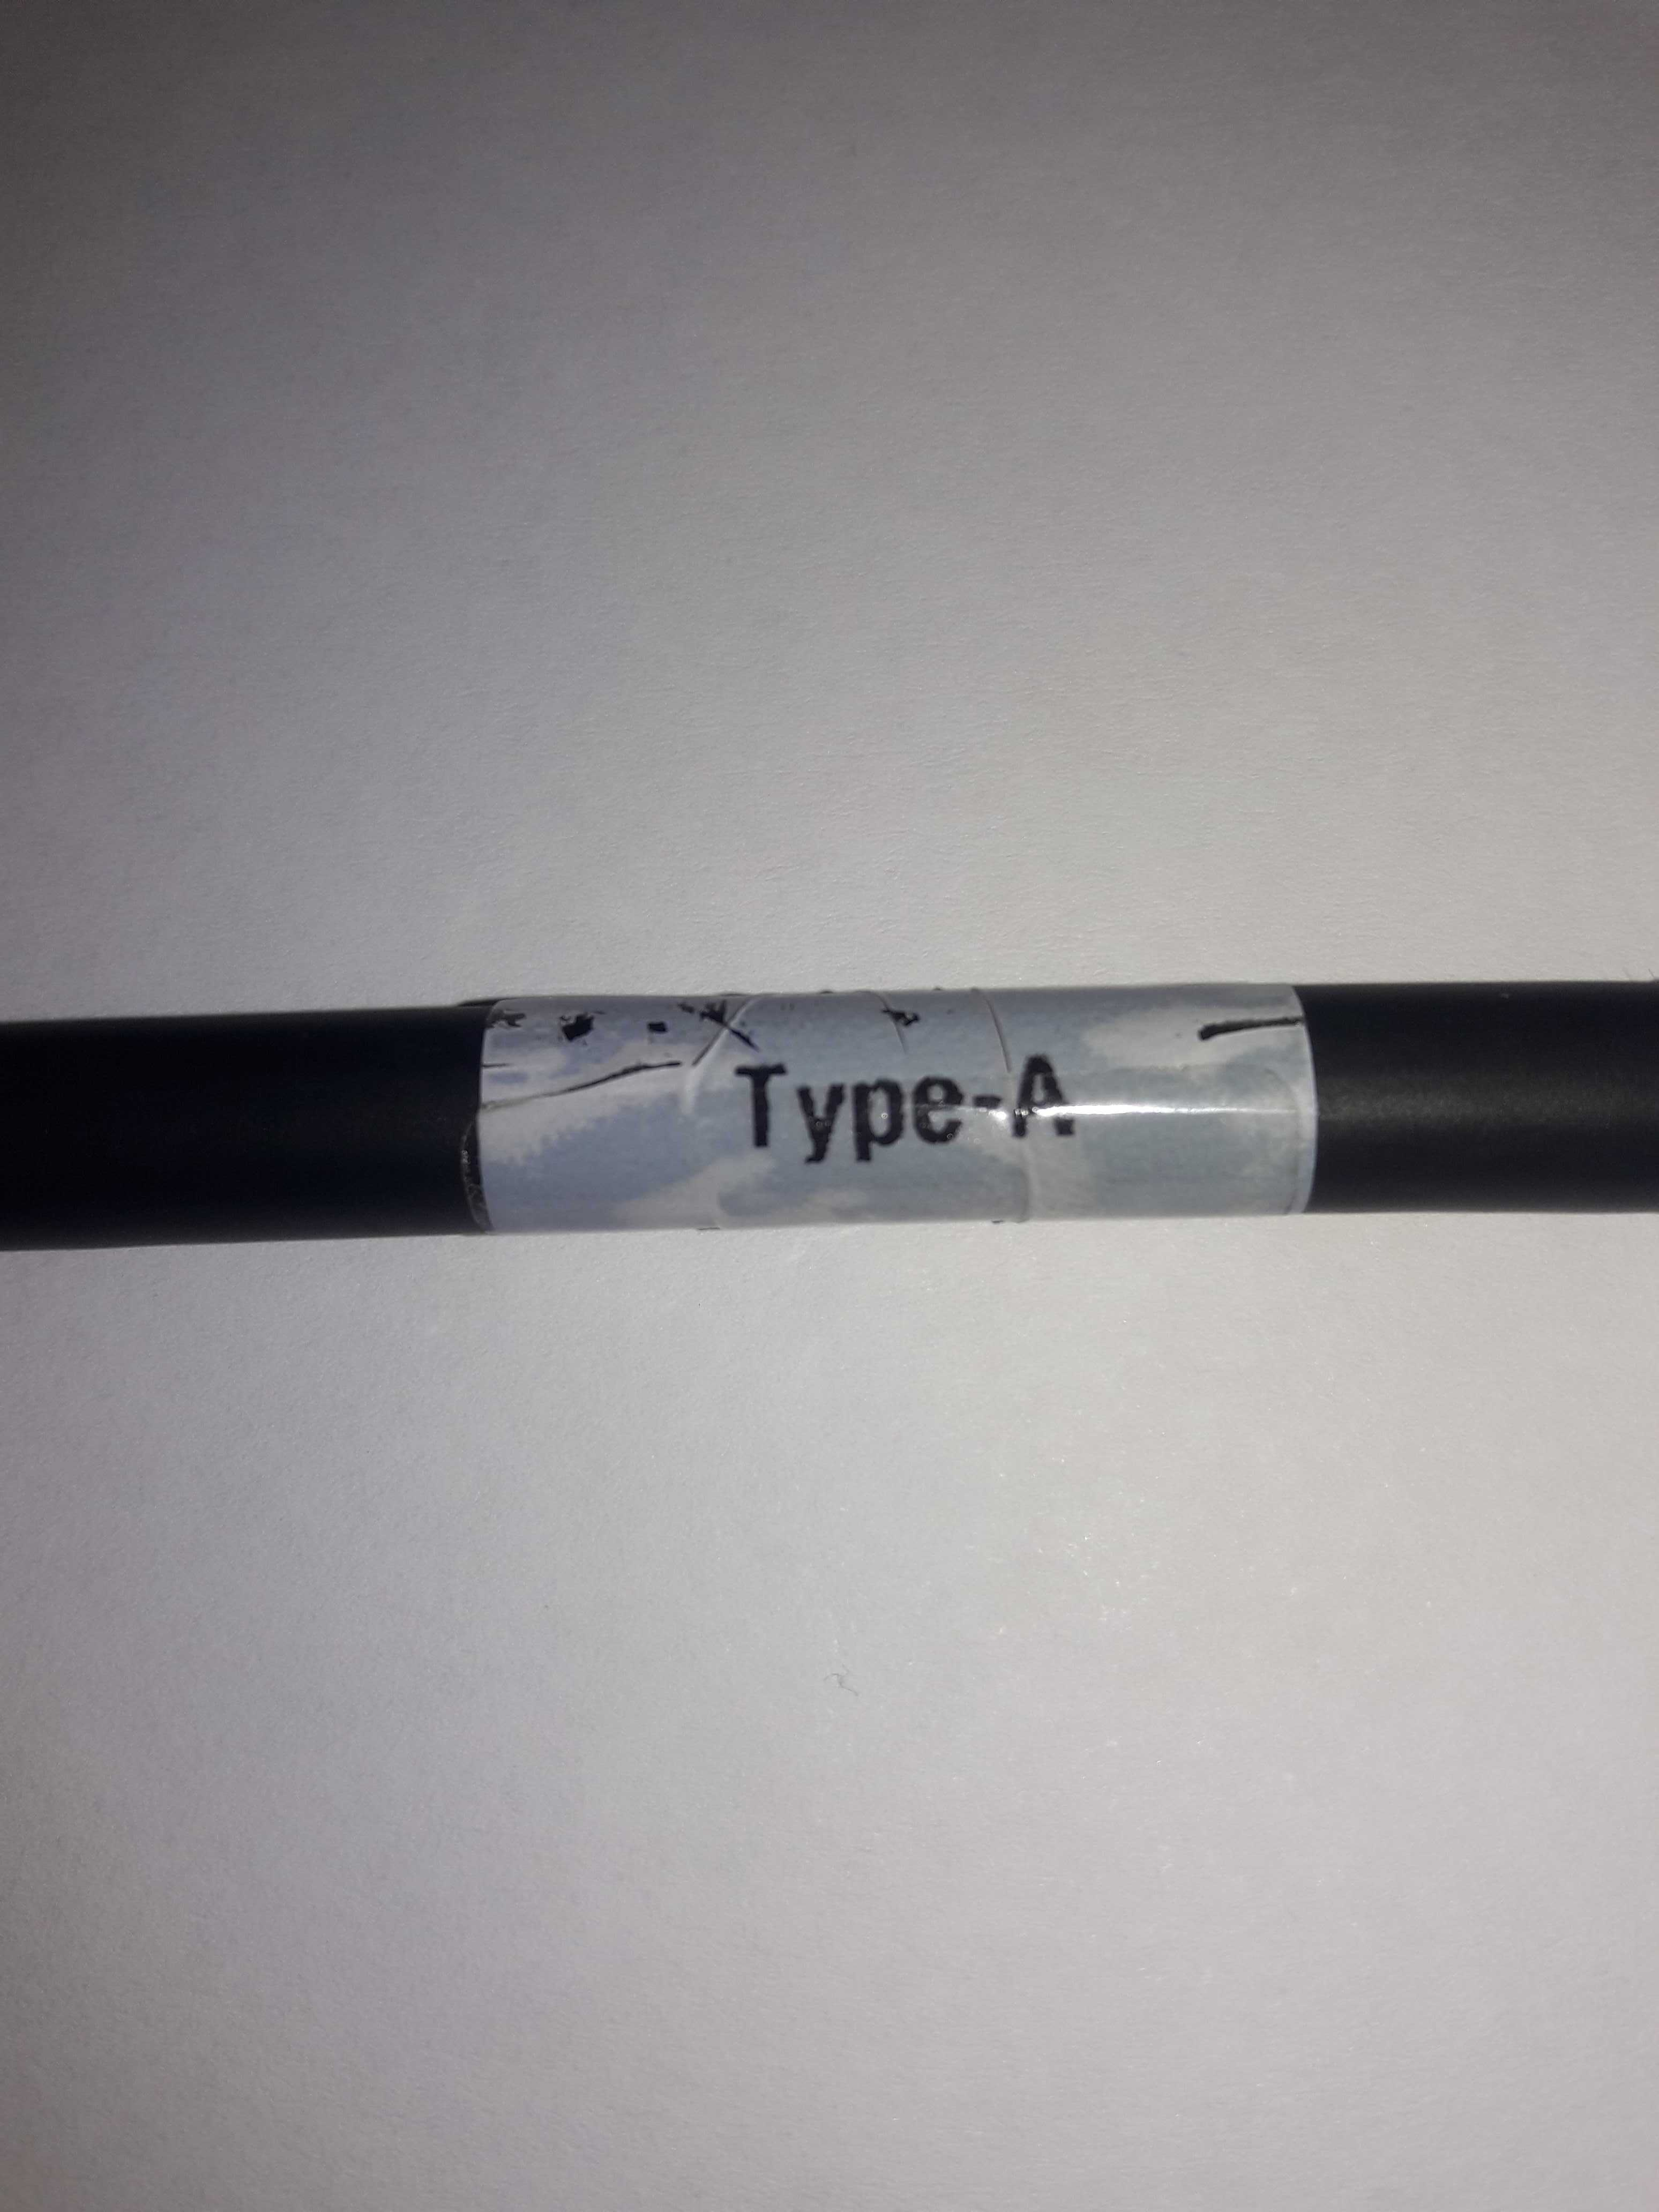
\includegraphics[width=\textwidth]{images/66.jpg}
  \end{subfigure}
  \hfill
  \begin{subfigure}{0.48\textwidth}
    \centering
    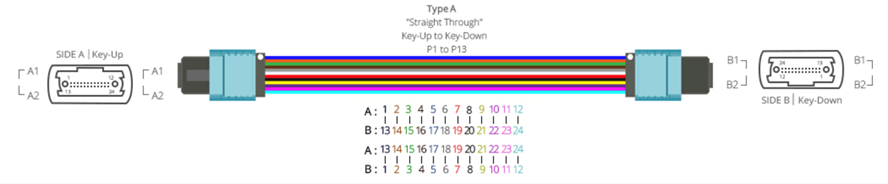
\includegraphics[width=\textwidth]{images/7.png}
  \end{subfigure}
\end{figure}

\newpage
\subsubsection{Adapter Keys}

  When we refer to the adapter key, it is a notch in the coupler that gives the connection orientation of the connectors. The polarities that are compatible with these adapters are Type A and Type B.

  1.) A Type A adapter or coupler polarity is (Key Up to Key Down)

  2.) A Type B adapter or coupler polarity is  (Key Up to Key Up).


  In this report, we will only document the Type A coupler.


\begin{figure}
  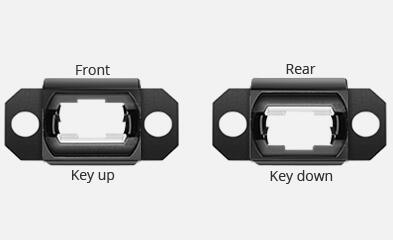
\includegraphics[width=11cm]{images/8.jpg}
  \centering
\end{figure}

\newpage
\subsubsection{Cable Connection Method}

  To connect these cables we will need to use the corresponding adapter for the polarity of the cable used. The image below illustrates the connection method used for a male-to-female type A cable using a coupler with Flange (Key Up to Down).

\begin{figure}
  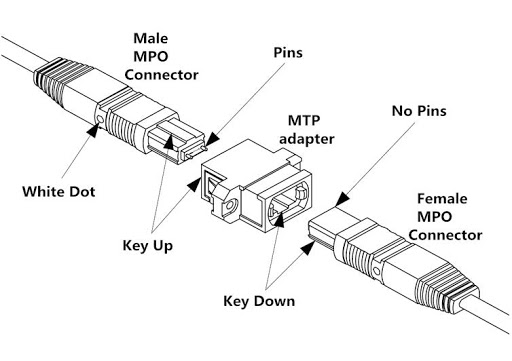
\includegraphics[width=11cm]{images/9.jpg}
  \centering
\end{figure}

\section{MTP / MPO cable acquisition method}

  Our MTP/MPO cables are supplied by a factory that specializes in fiber optic materials and structured cabling. We have been working with this company throughout the construction period of the telescope at Rubin, providing us with network cables, fiber optic cables, specific tools, and any other material related to structured cabling. One of the advantages that we have working with this company is that we have direct contact with a representative allowing us to place special orders or requests for a specific type of material we would like to work with satisfying our needs.


\subsection{Purchase Method}

  To purchase a specific cable we need to know the type of cable we would like to use, its polarity, and any other feature required. Once all of this information is gathered a company representative is contacted with our requirements and the order is received and processed. The company then proceed to manufacture the cable and Is shipped to Tucson and later to Chile which is received by the IT Team at the AURA Facility all in approximately 2 months.

  We made our first purchase for an MTP / MPO cable with military protection to perform a stress test of the material along with its durability.

\section{Installation and maintenance time of the MTP / MPO cable}

  To carry out the installation of the cables, we first need to request authorization within a week in advance to the managers and safety personnel in charge, this whole process is documented on a ticket in Jira. For each day of the work, IT has to fill out a daily activity registration form to document the activities that will be carried out for that particular day of work. This form is then delivered to Rubin Safety personnel who are in charge of authorizing the activity and supervising the work done for any safety hazard.

  Each area of work has to be demarcated with cones along with an informative table showing the person's name in charge of the work and the areas that will be closed throughout the work period. IT also has to notify Rubin personnel by radio on channel 3 that work will take place in the area authorized.

  The installation of this type of cable can usually take up to 2 days with a workgroup composed of 4 members but maintenance can take up to 3 workdays with the same amount of people, this is because the IT Team has to specifically check and withdraw each cable, taking into account the following considerations.

  First, we have to locate the cable we are going to be doing maintenance on or replacing.
  Remove the cable from where it's currently installed and located.
  Prepare and install the new cable in replacement for the one that was removed.


  Note: The times provided above are all estimates taking into consideration that the cables are installed in the computer room in rack B7 and extend to the sixth floor of the pier.

\newpage
\subsection{MTP cable routing analysis}

\begin{figure}
  \centering
  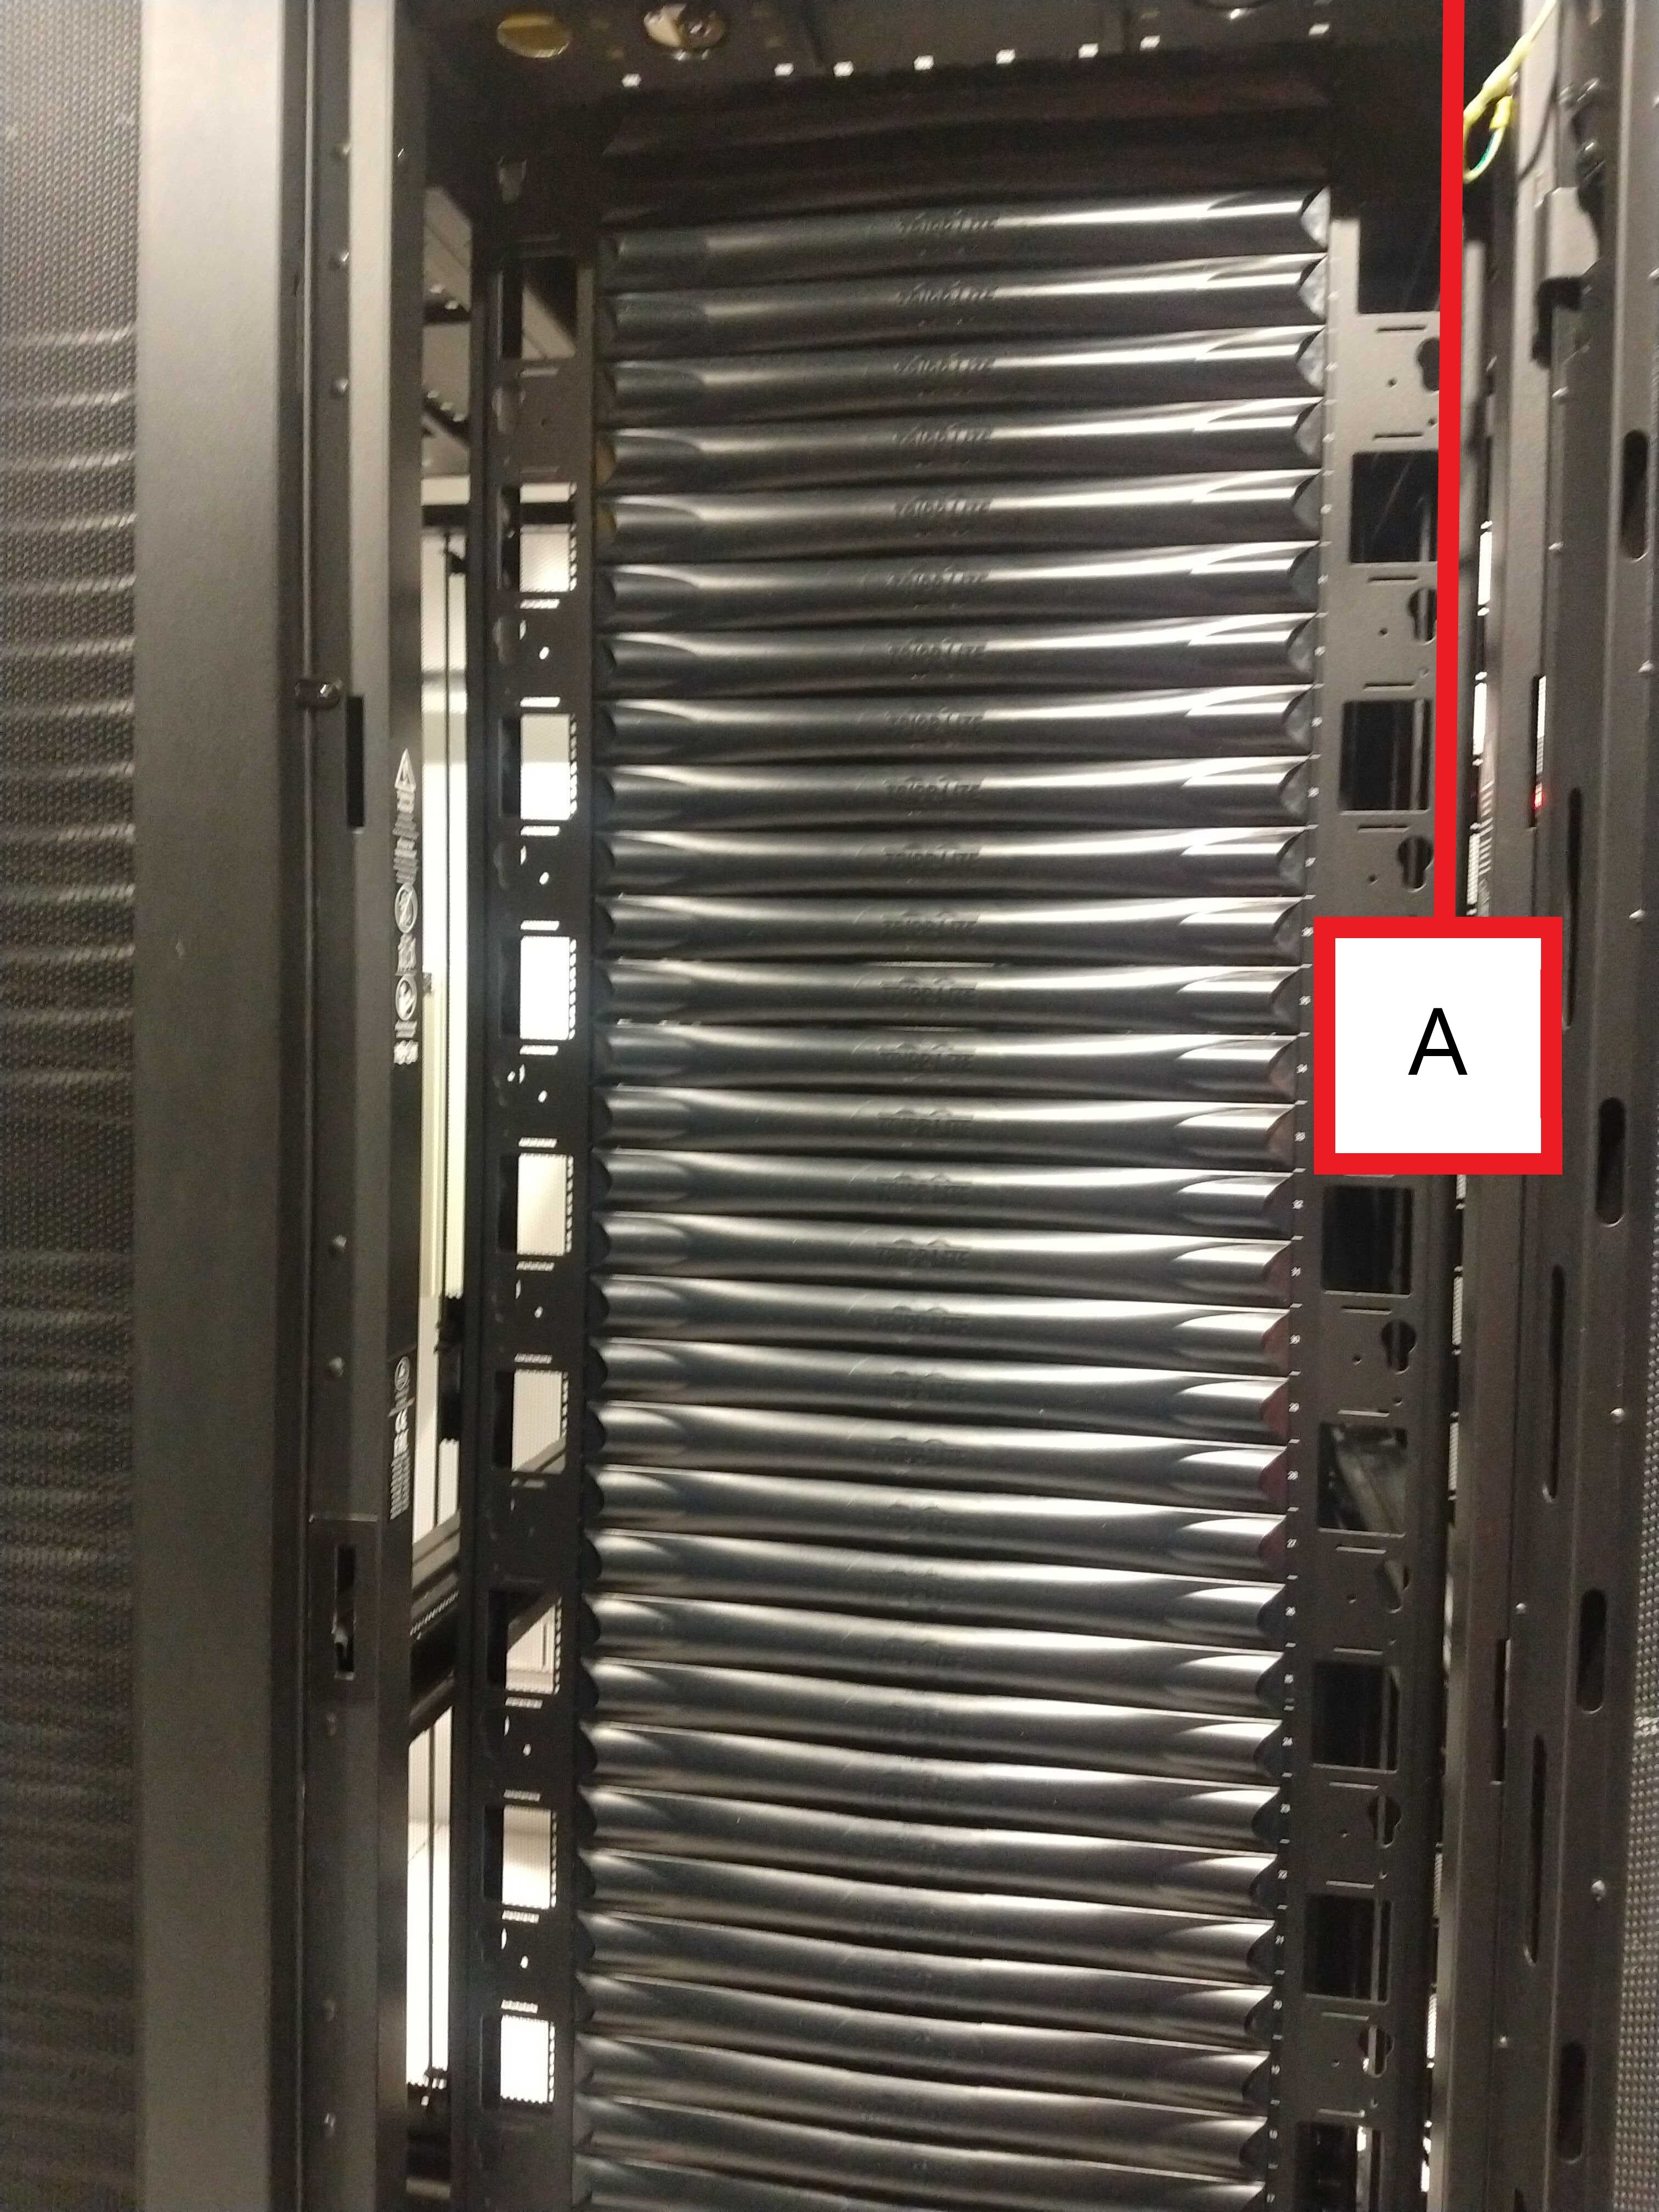
\includegraphics[width=9cm]{images/111.jpg}
  \caption*{The DAQ rack will be located in the datacenter at Pachon.} 
\end{figure}
  

\newpage

\begin{figure}
  \centering
  \begin{subfigure}{0.40\textwidth}
    \centering
    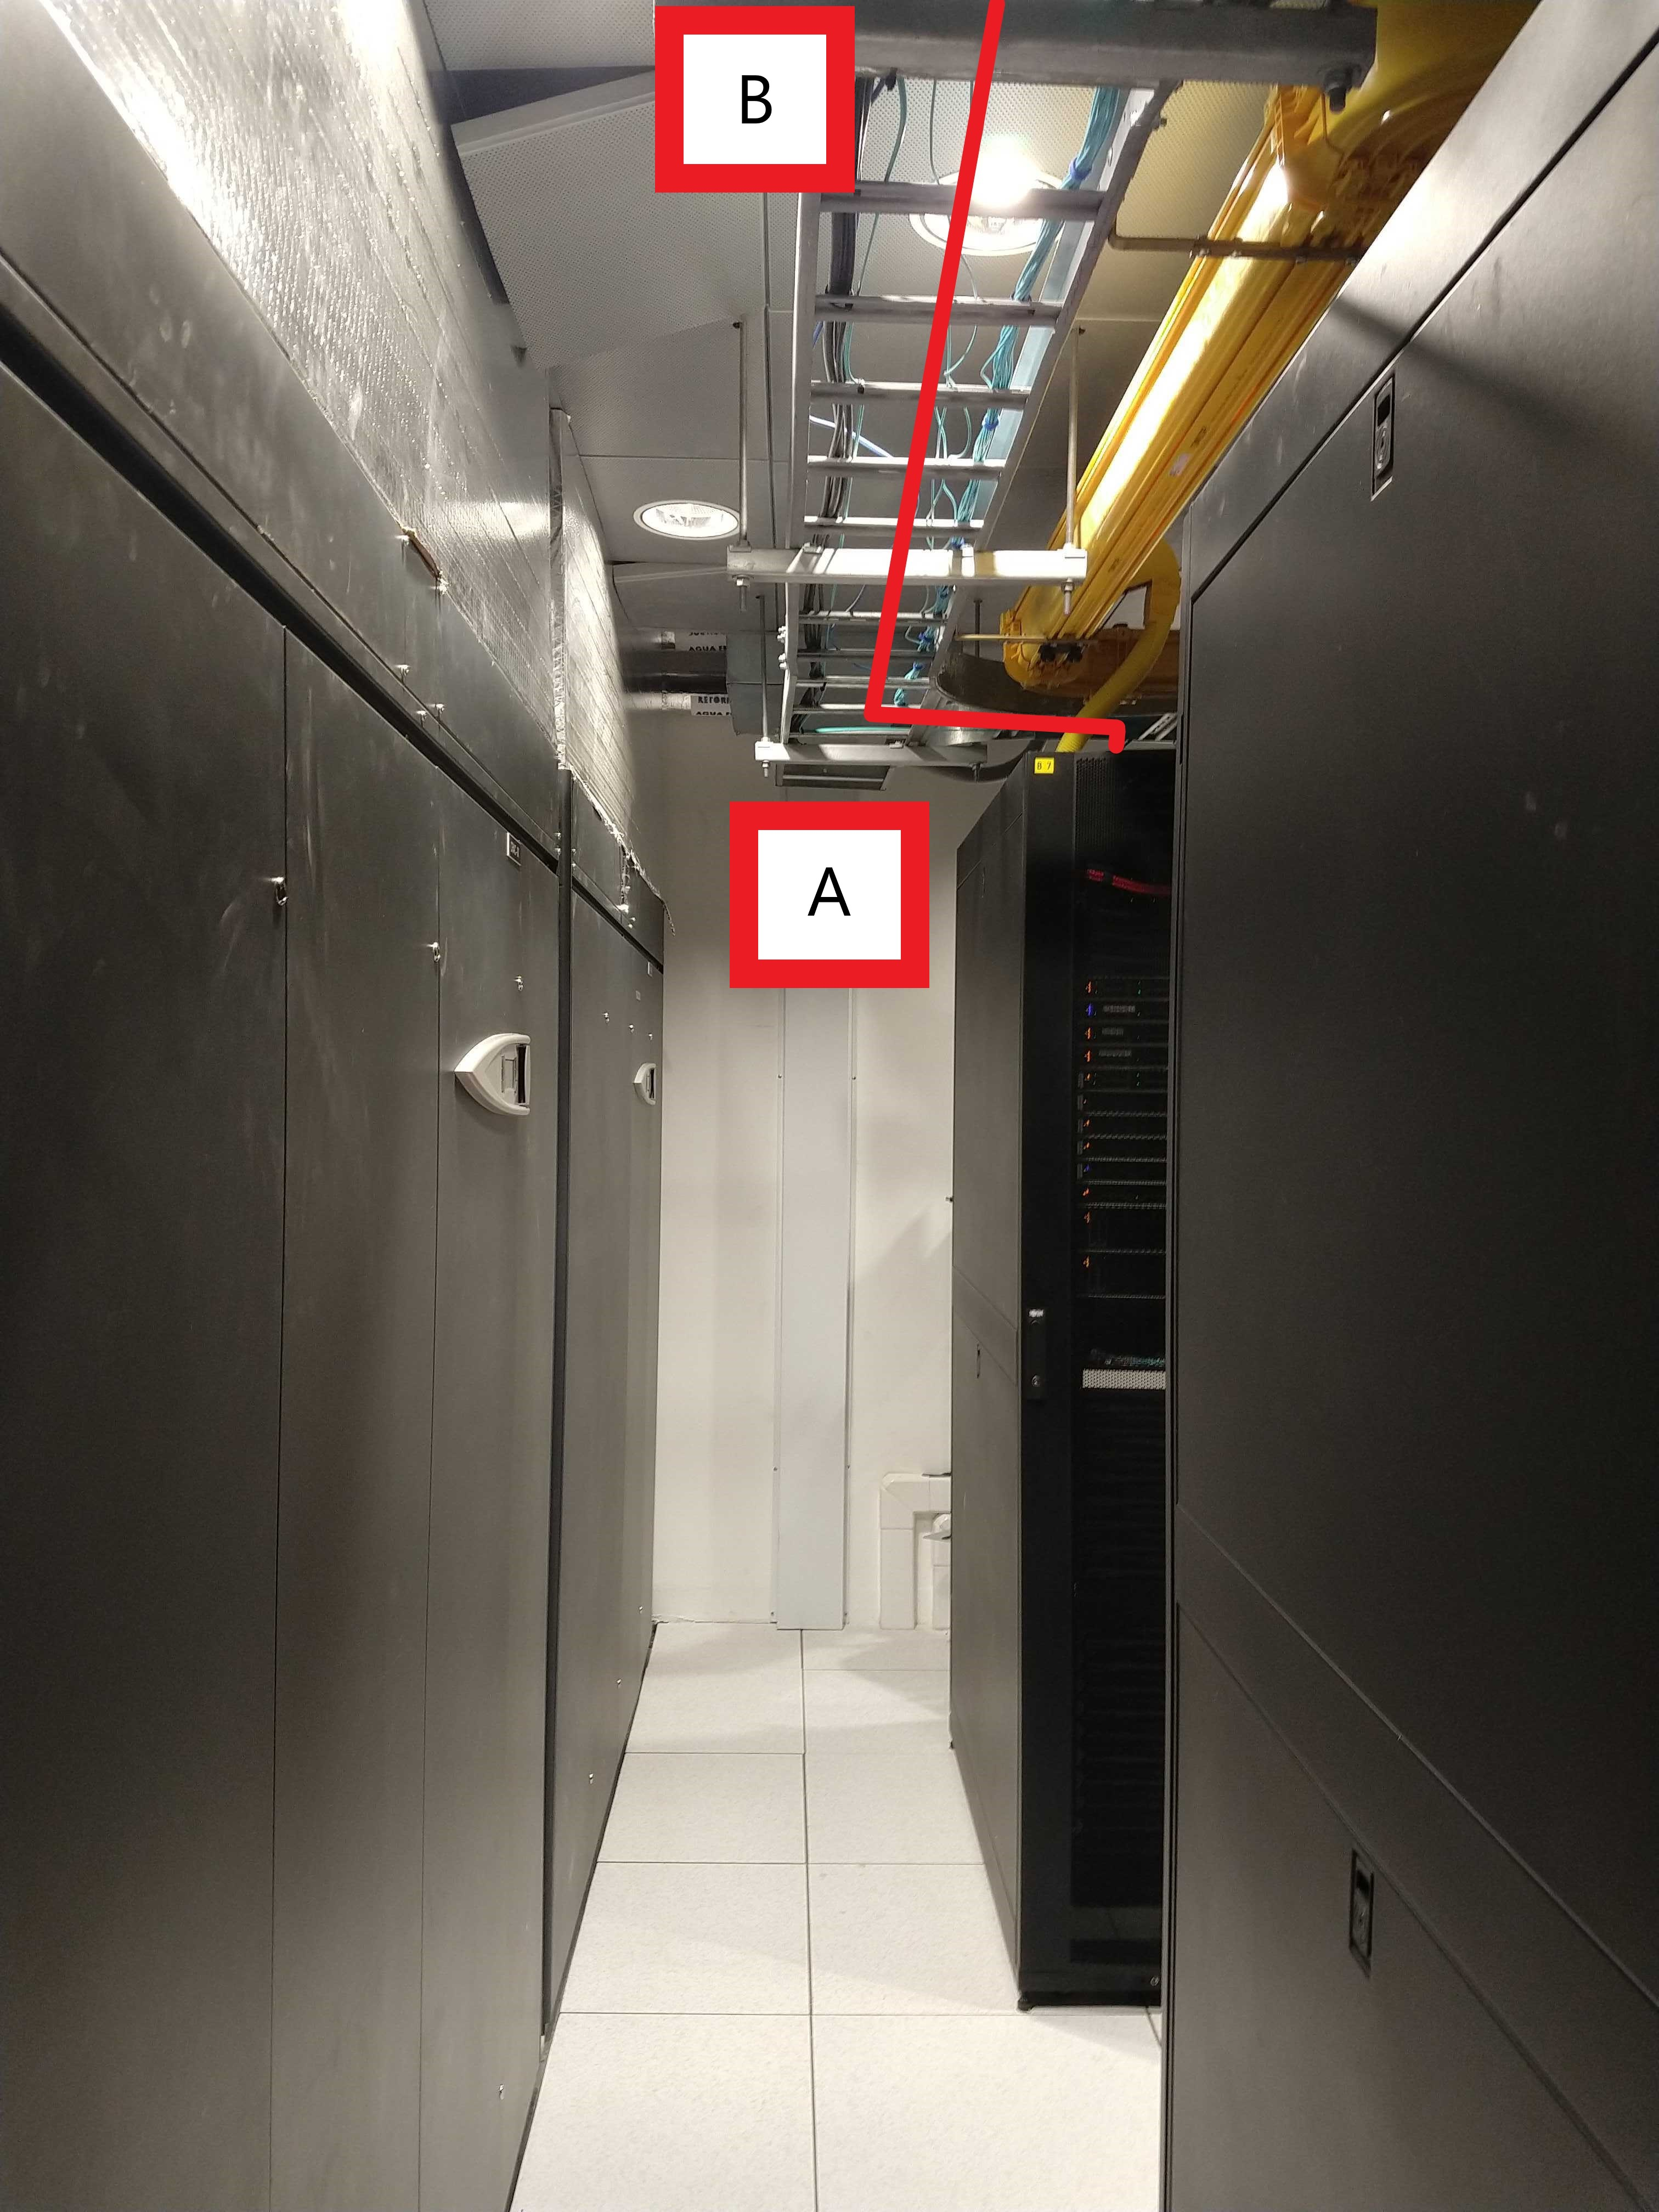
\includegraphics[width=\textwidth]{images/11.jpg}
  \end{subfigure}
  \hfill
  \begin{subfigure}{0.40\textwidth}
    \centering
    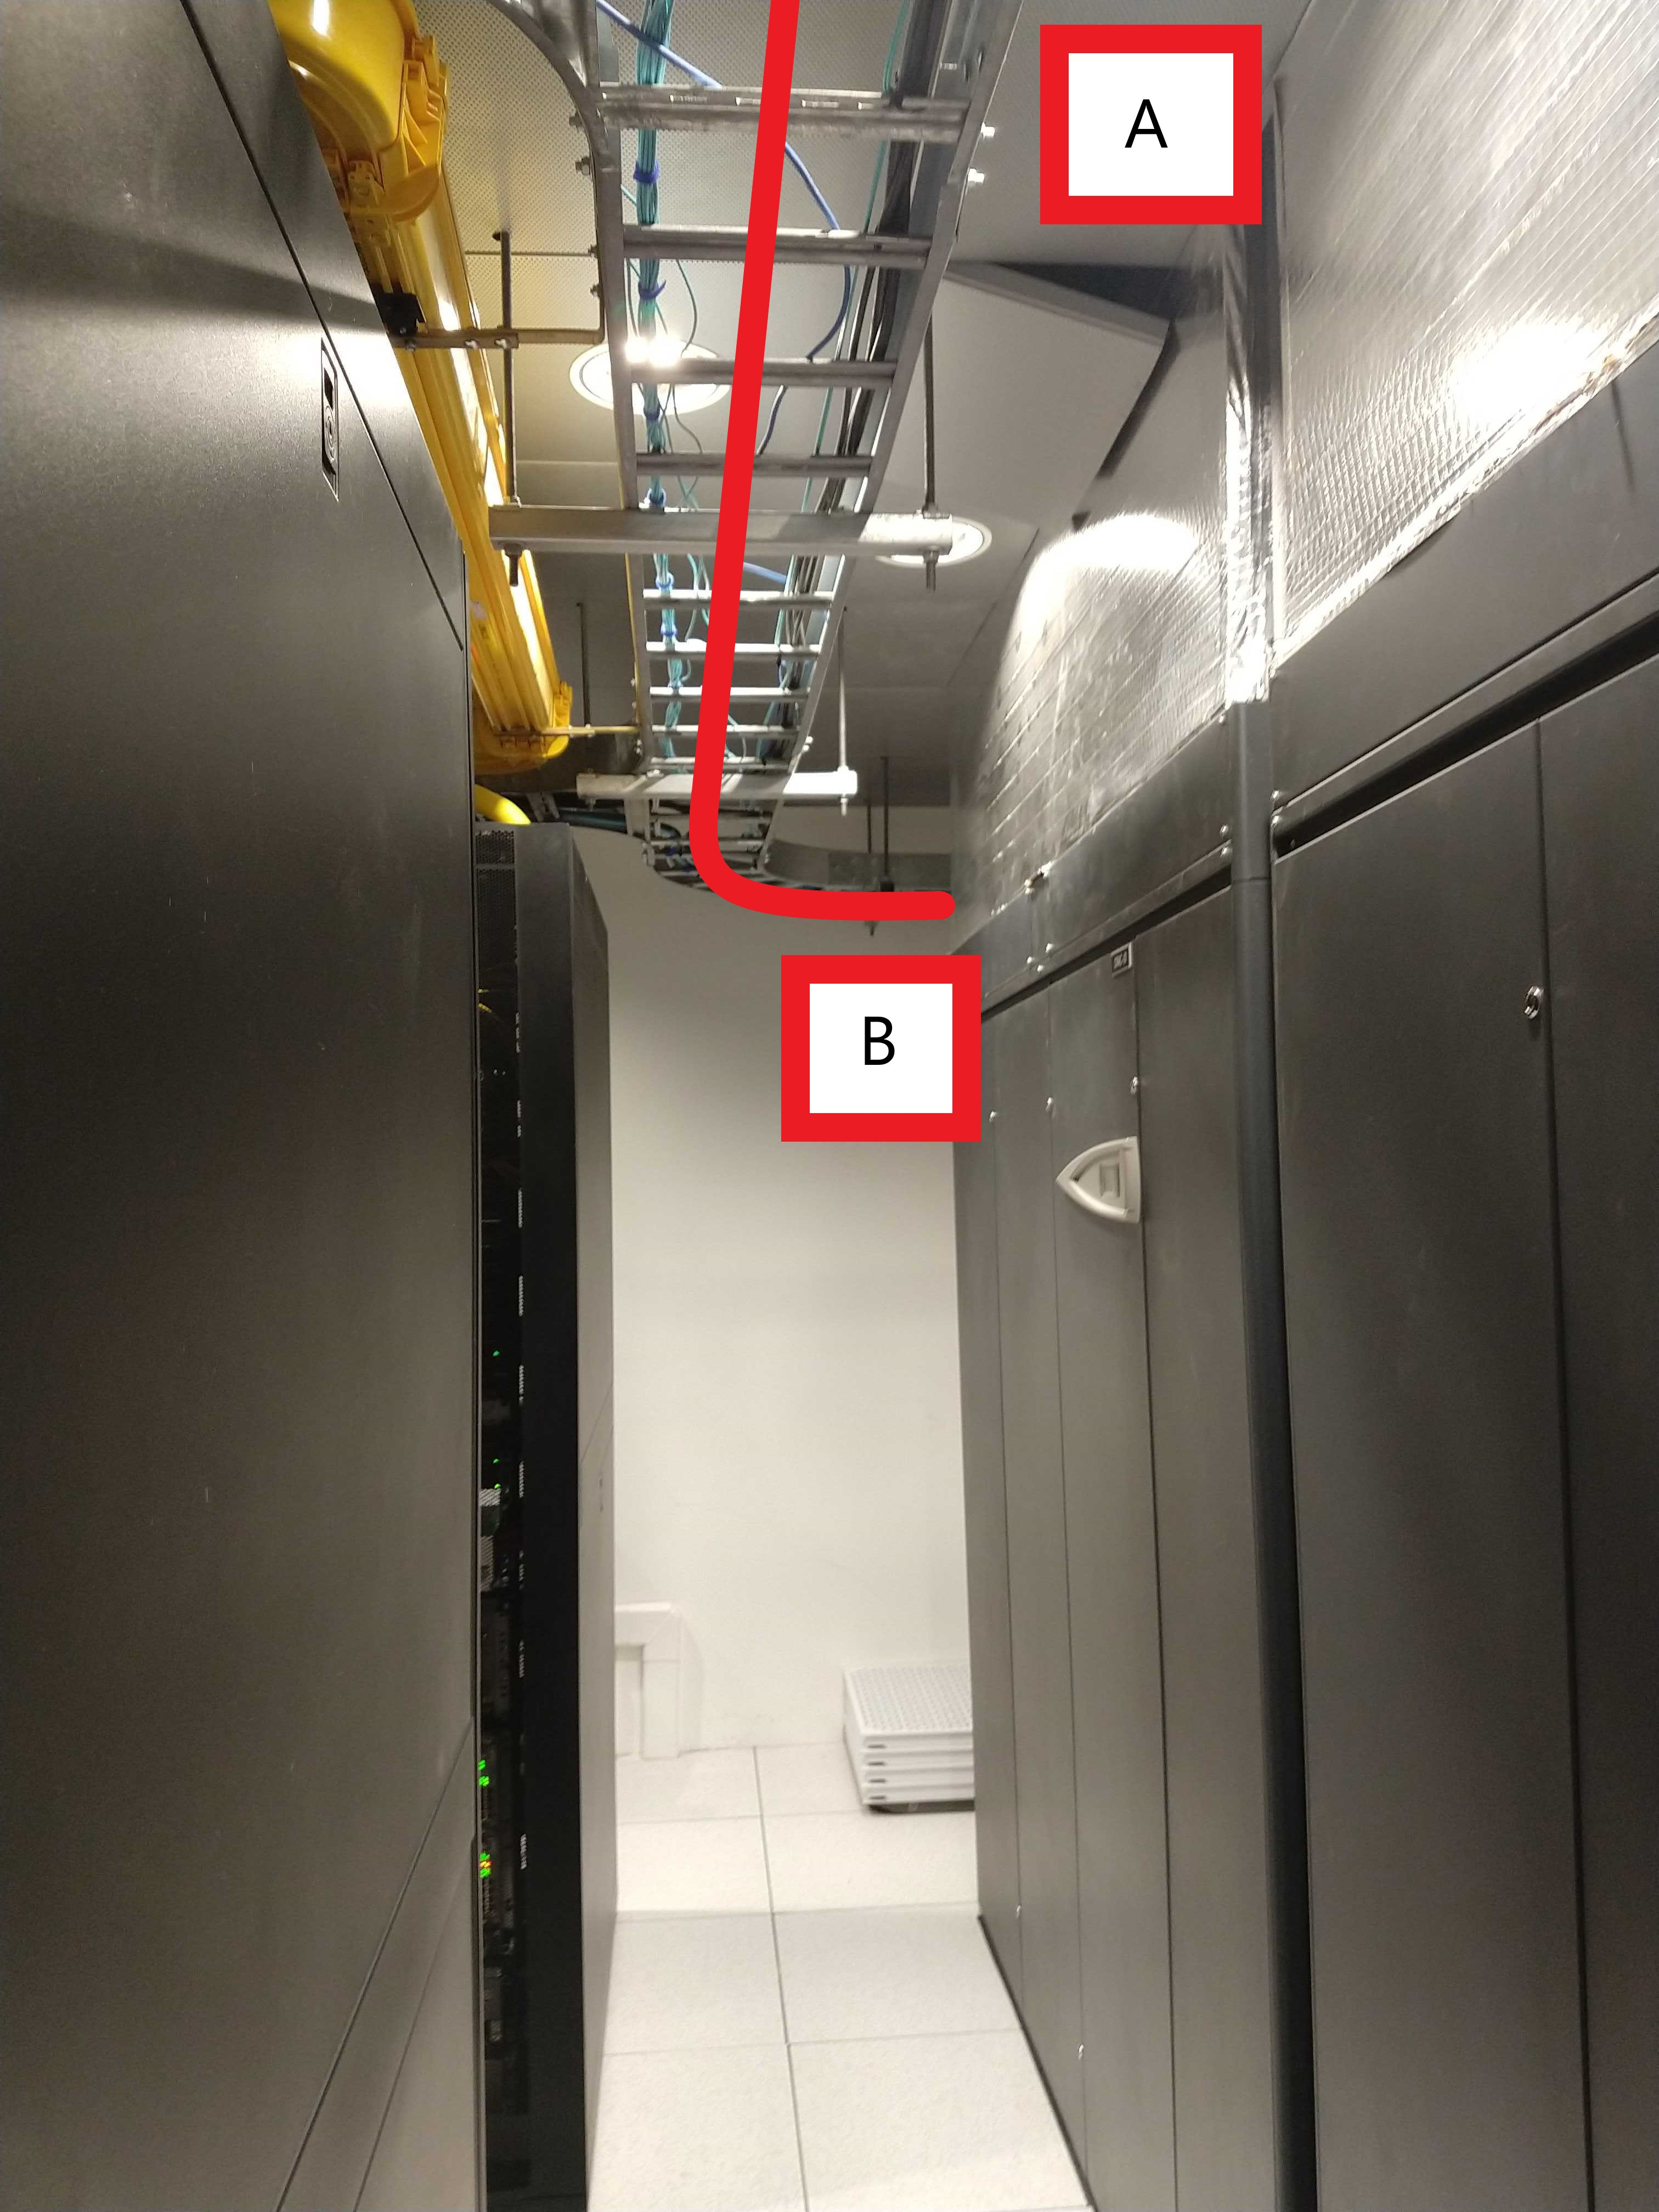
\includegraphics[width=\textwidth]{images/12.jpg}
  \end{subfigure}
\end{figure}

The cable originates and exists out of the top of rack B7 at position A of the computer room.The cable then runs through the cable tray in the same room to position B of the computerroom exiting at the end of the room

\begin{figure}
  \centering
  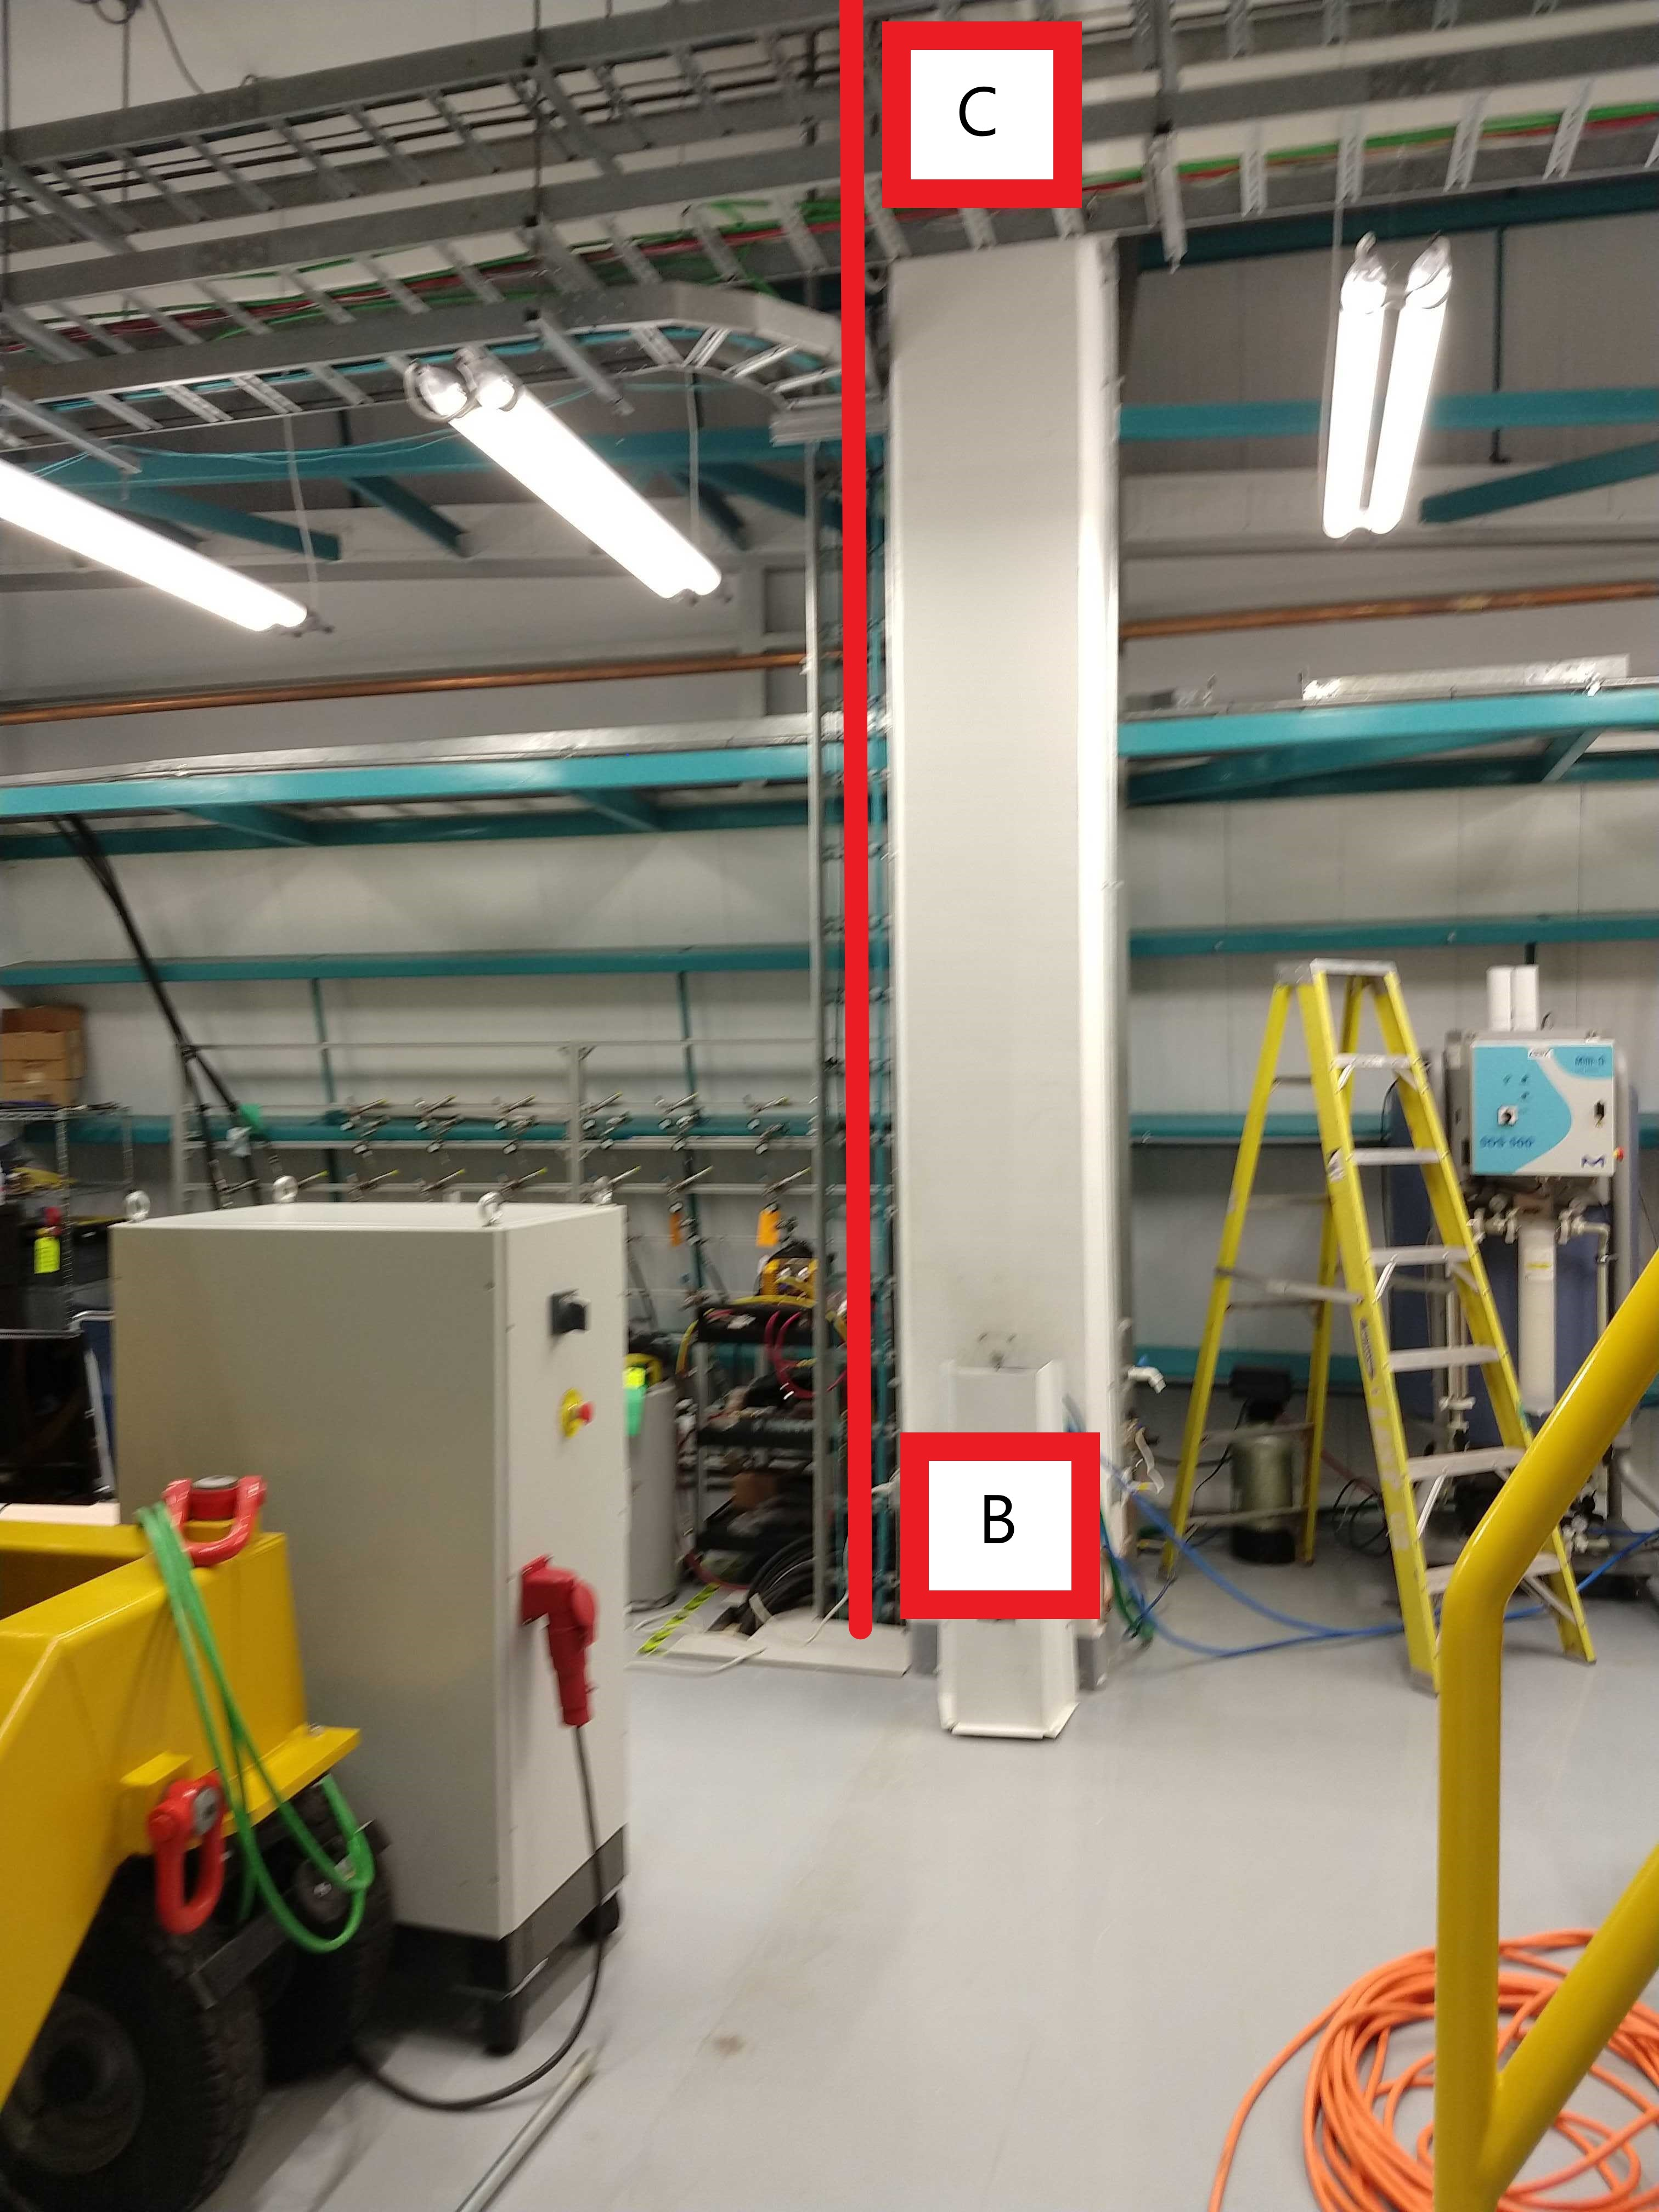
\includegraphics[width=6cm]{images/13.jpg}
\end{figure}

The cable then appears on the cable tray of the third floor and runs along the pillar to point C extending to the floor above.

\begin{figure}
  \centering
  \begin{subfigure}{0.45\textwidth}
    \centering
    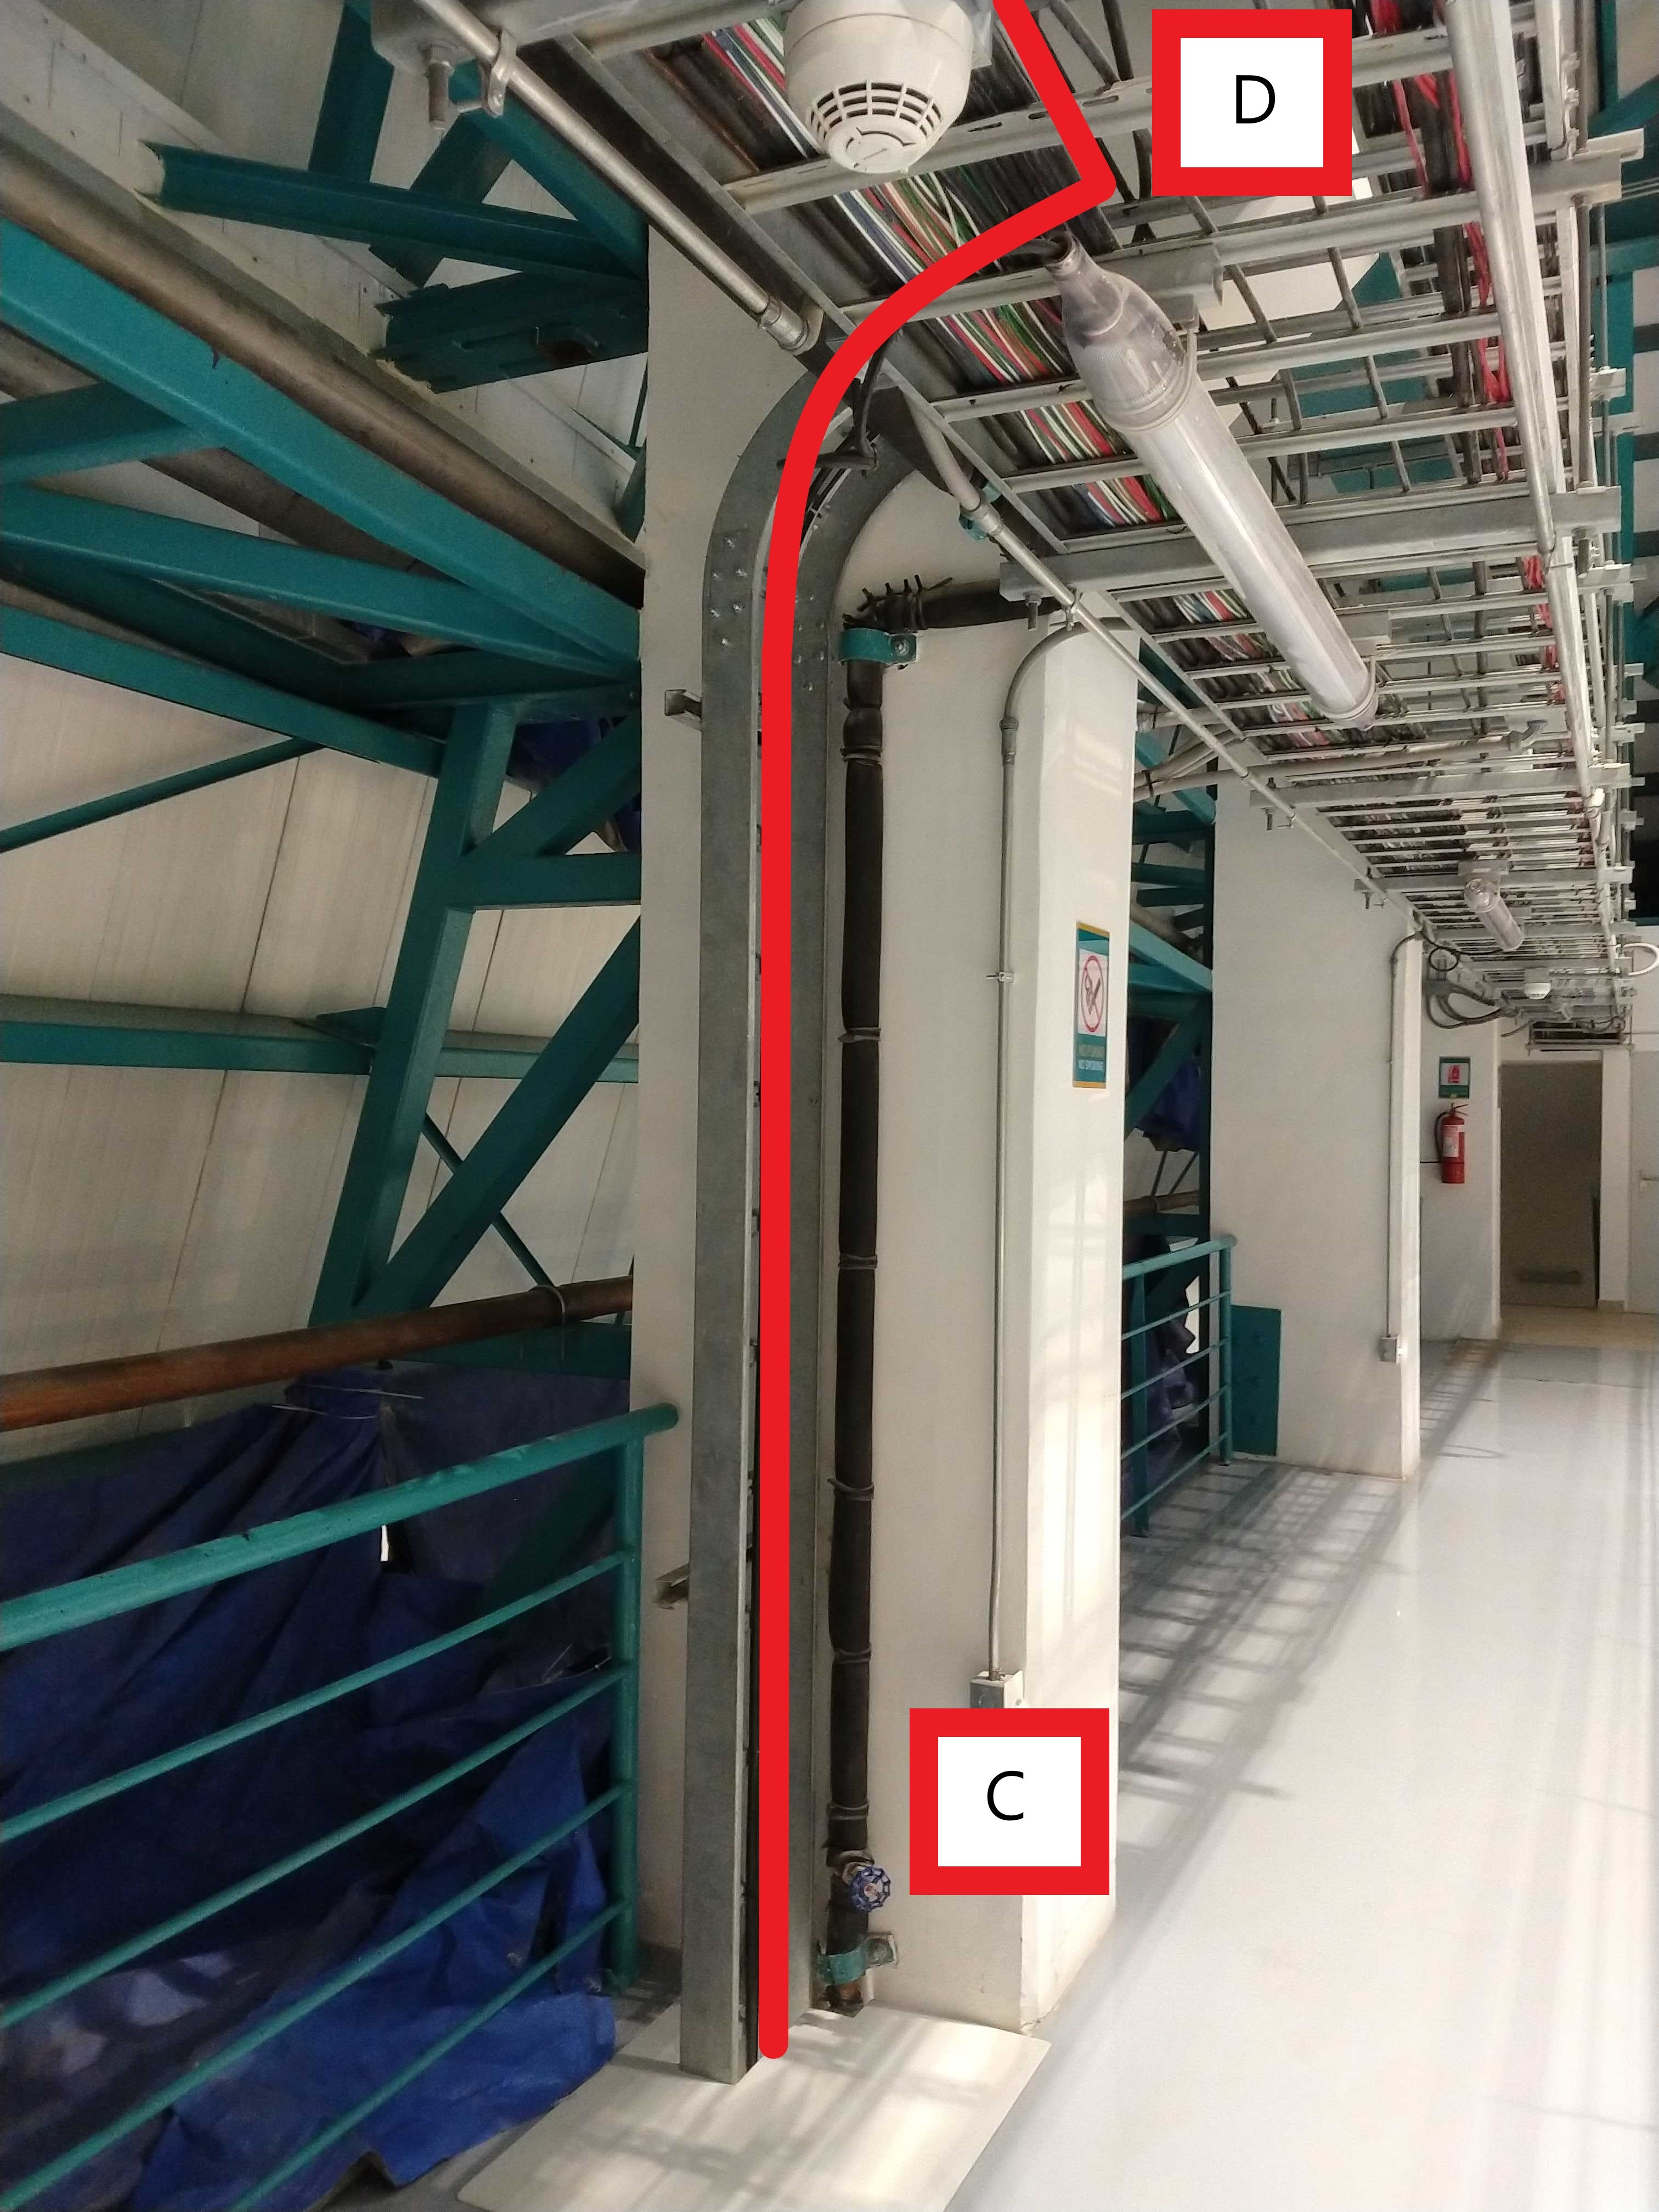
\includegraphics[width=\textwidth]{images/14.jpg}
  \end{subfigure}
  \hfill
  \begin{subfigure}{0.45\textwidth}
    \centering
    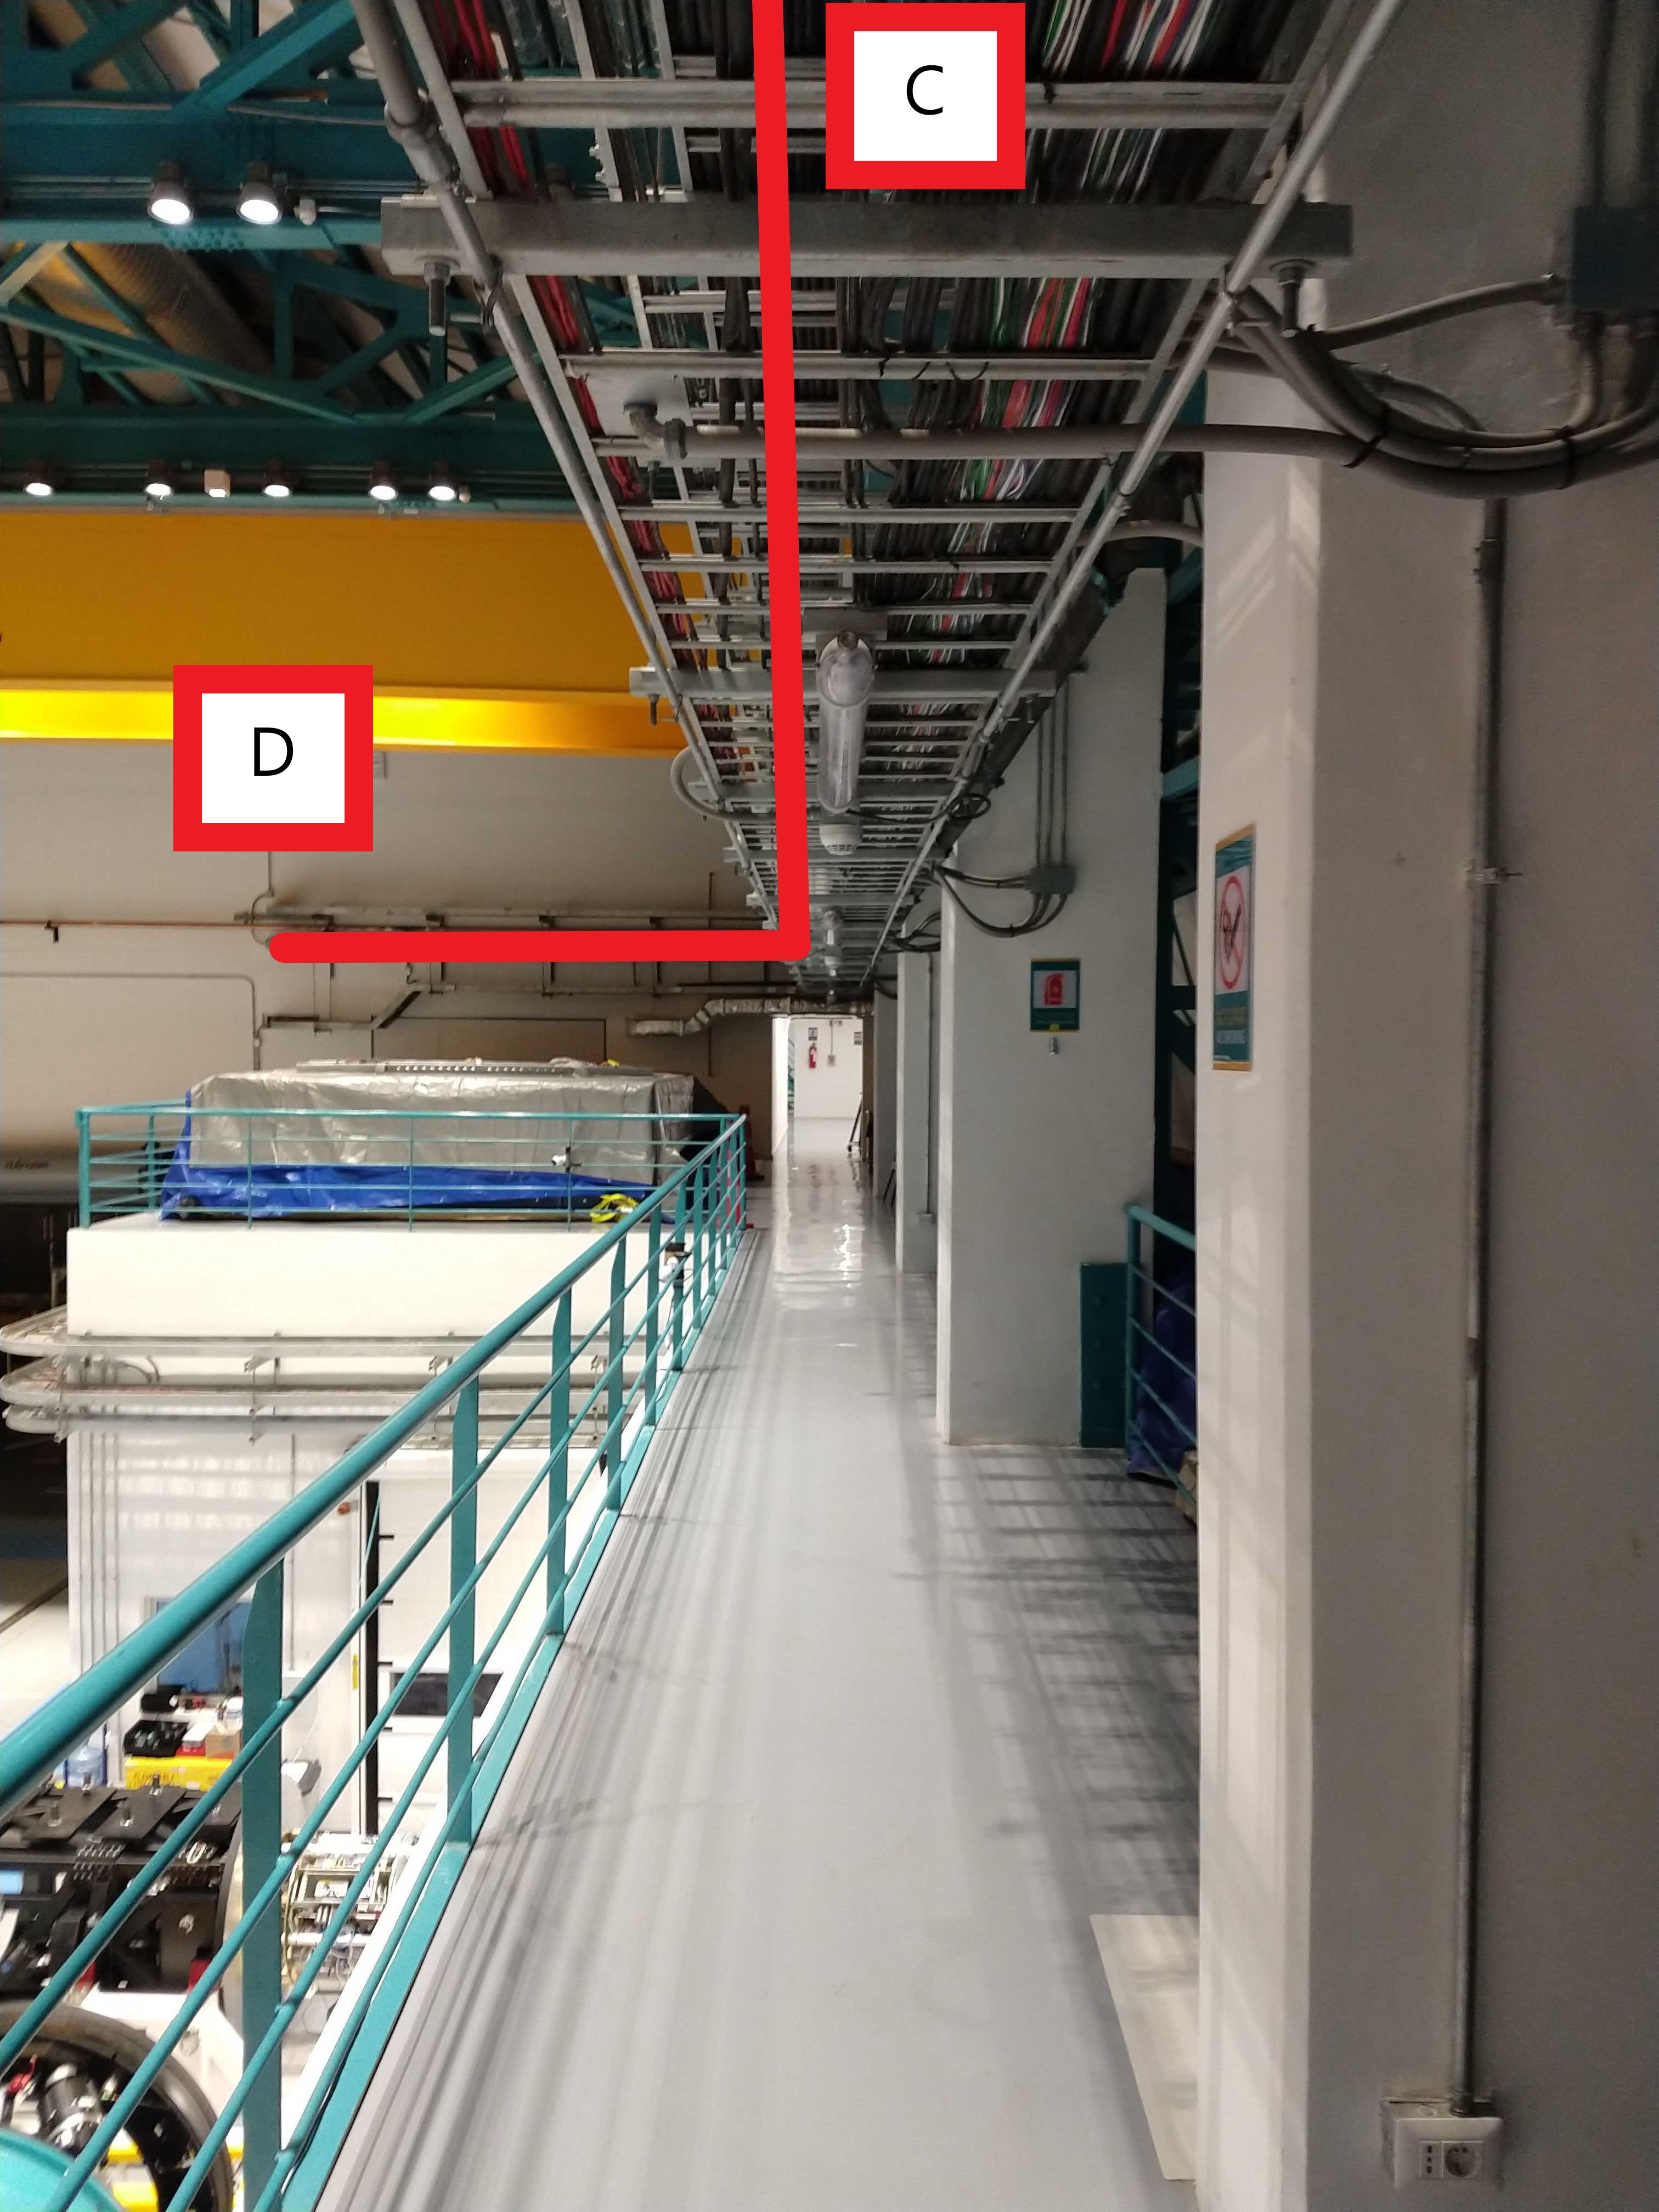
\includegraphics[width=\textwidth]{images/15.jpg}
  \end{subfigure}
\end{figure}
   
\begin{figure}
  \centering
  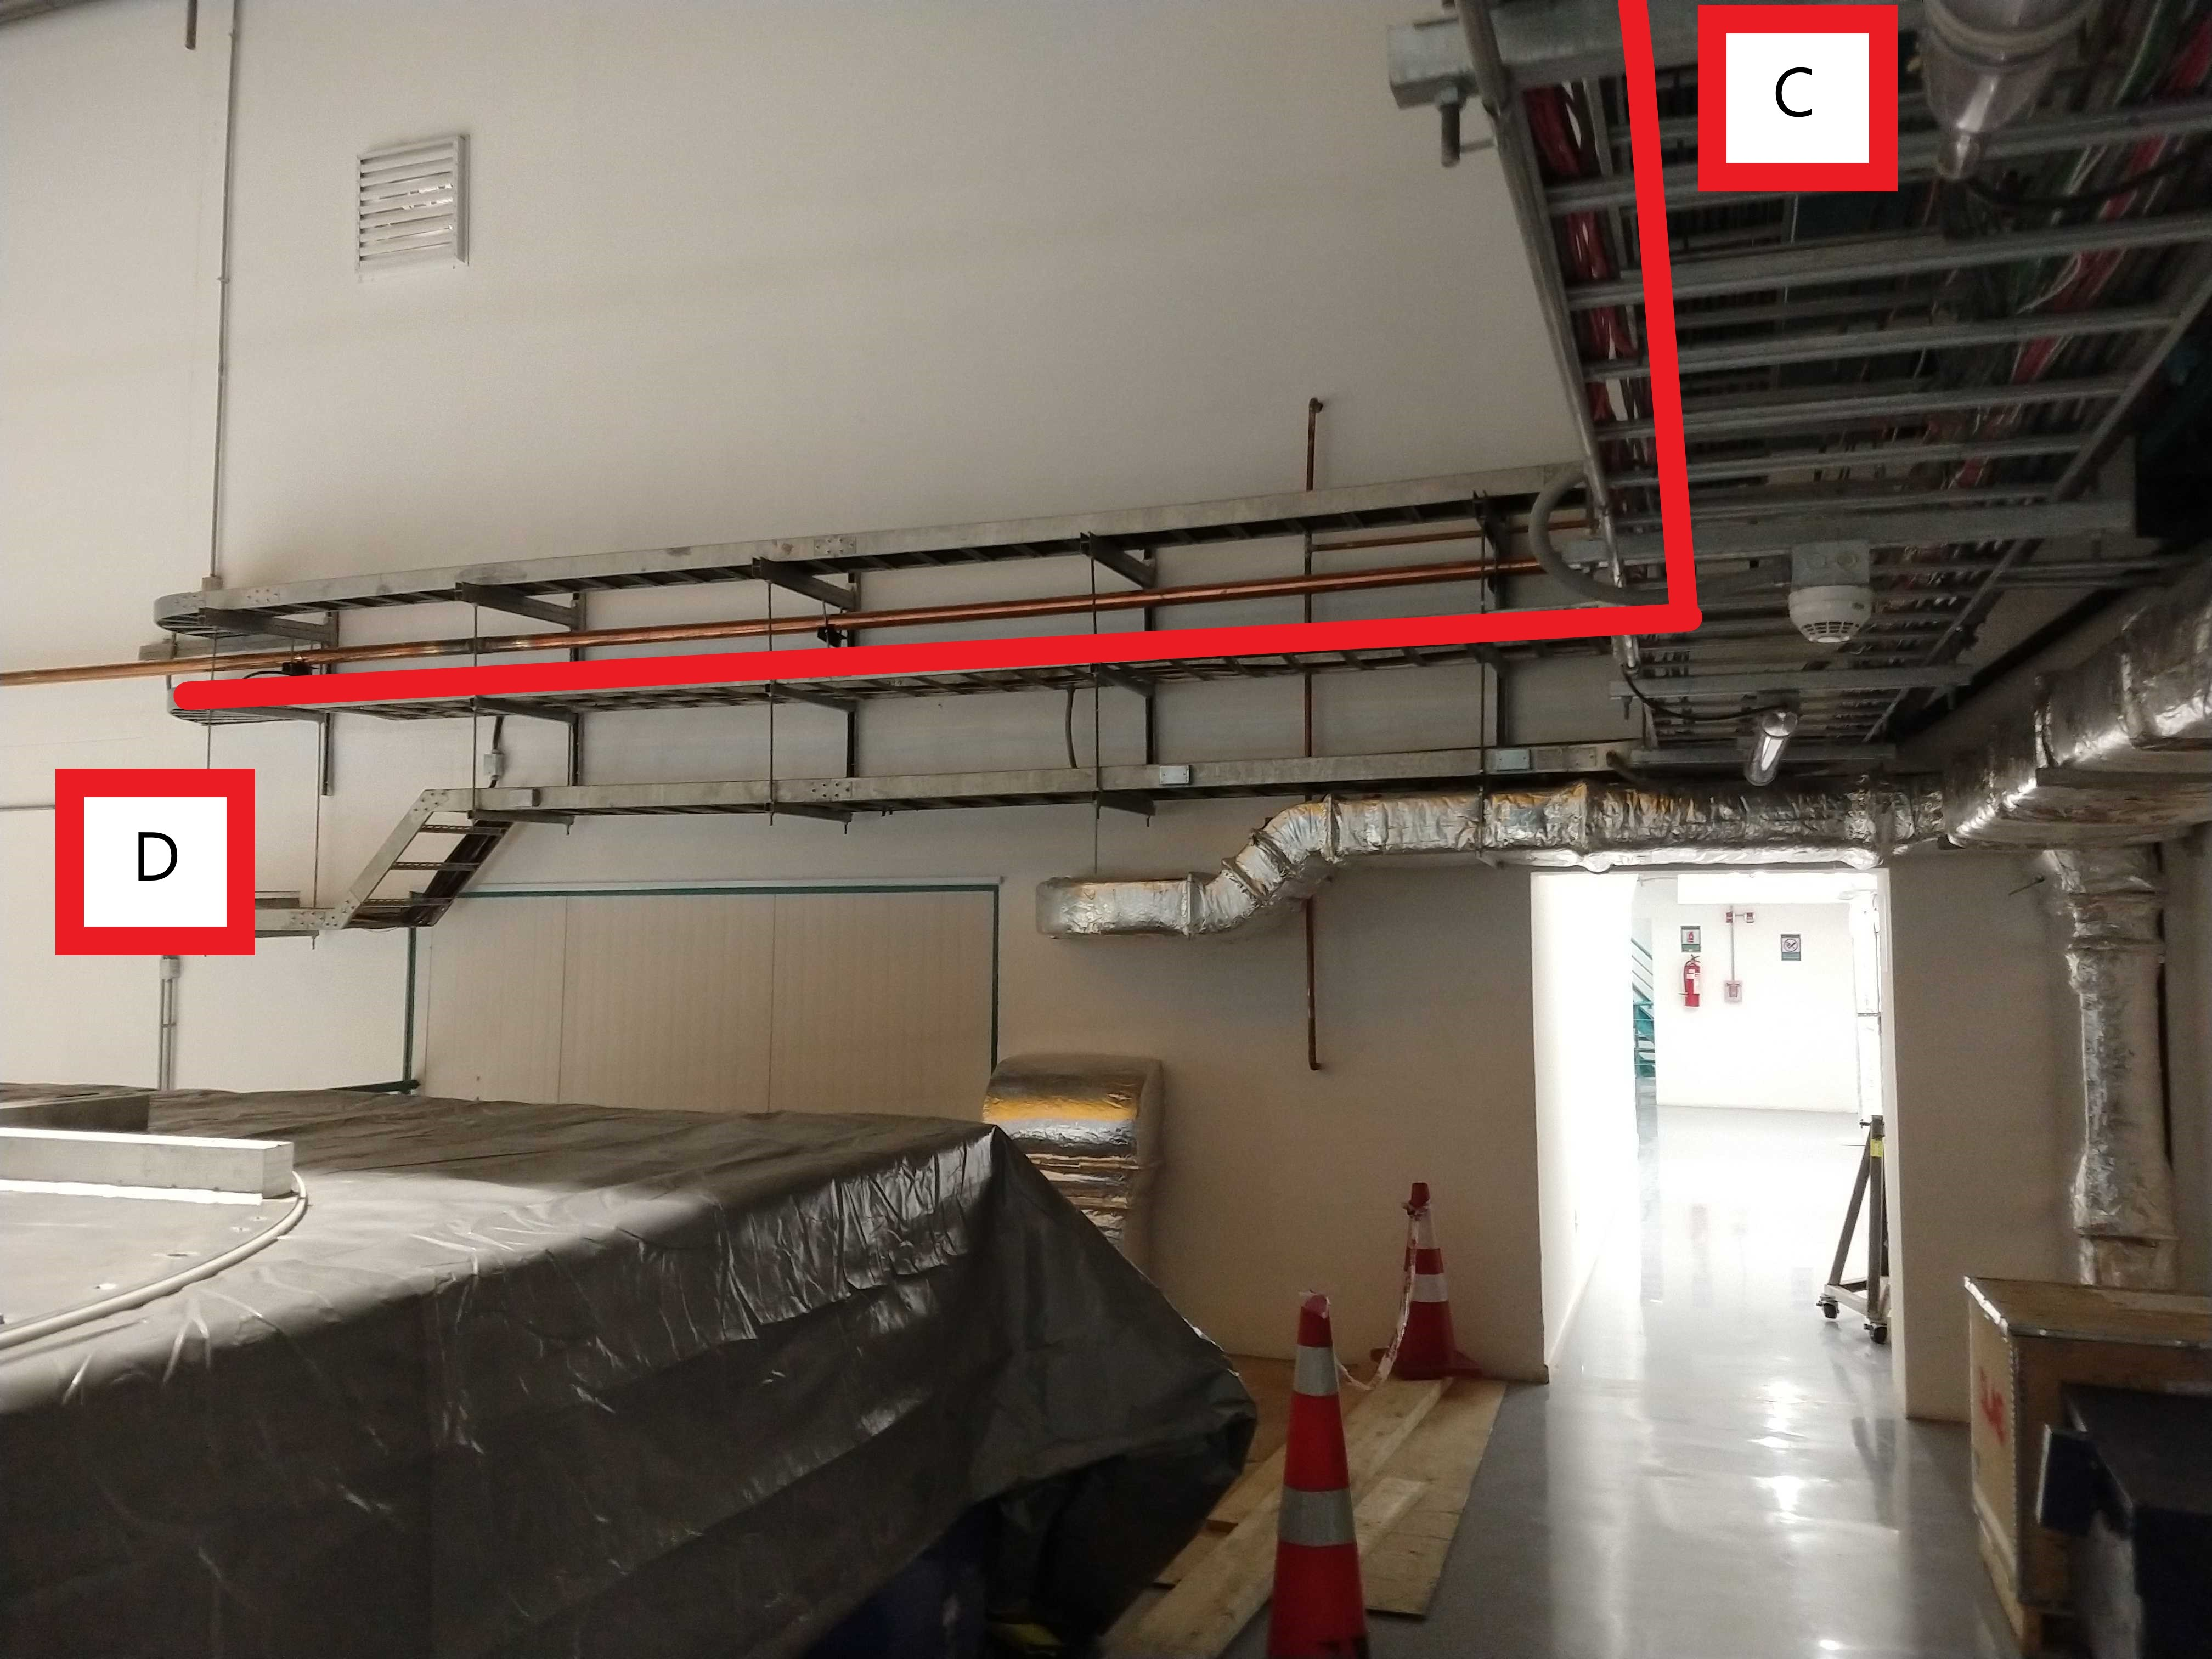
\includegraphics[width=10cm]{images/16.jpg}
  \caption*{The cable shows up again on the fourth floor of the main building and connects to the cable tray found on the same floor, the cable then follows the path of the cable tray connecting to point D.}
\end{figure}

  
\newpage

\begin{figure}
  \centering
  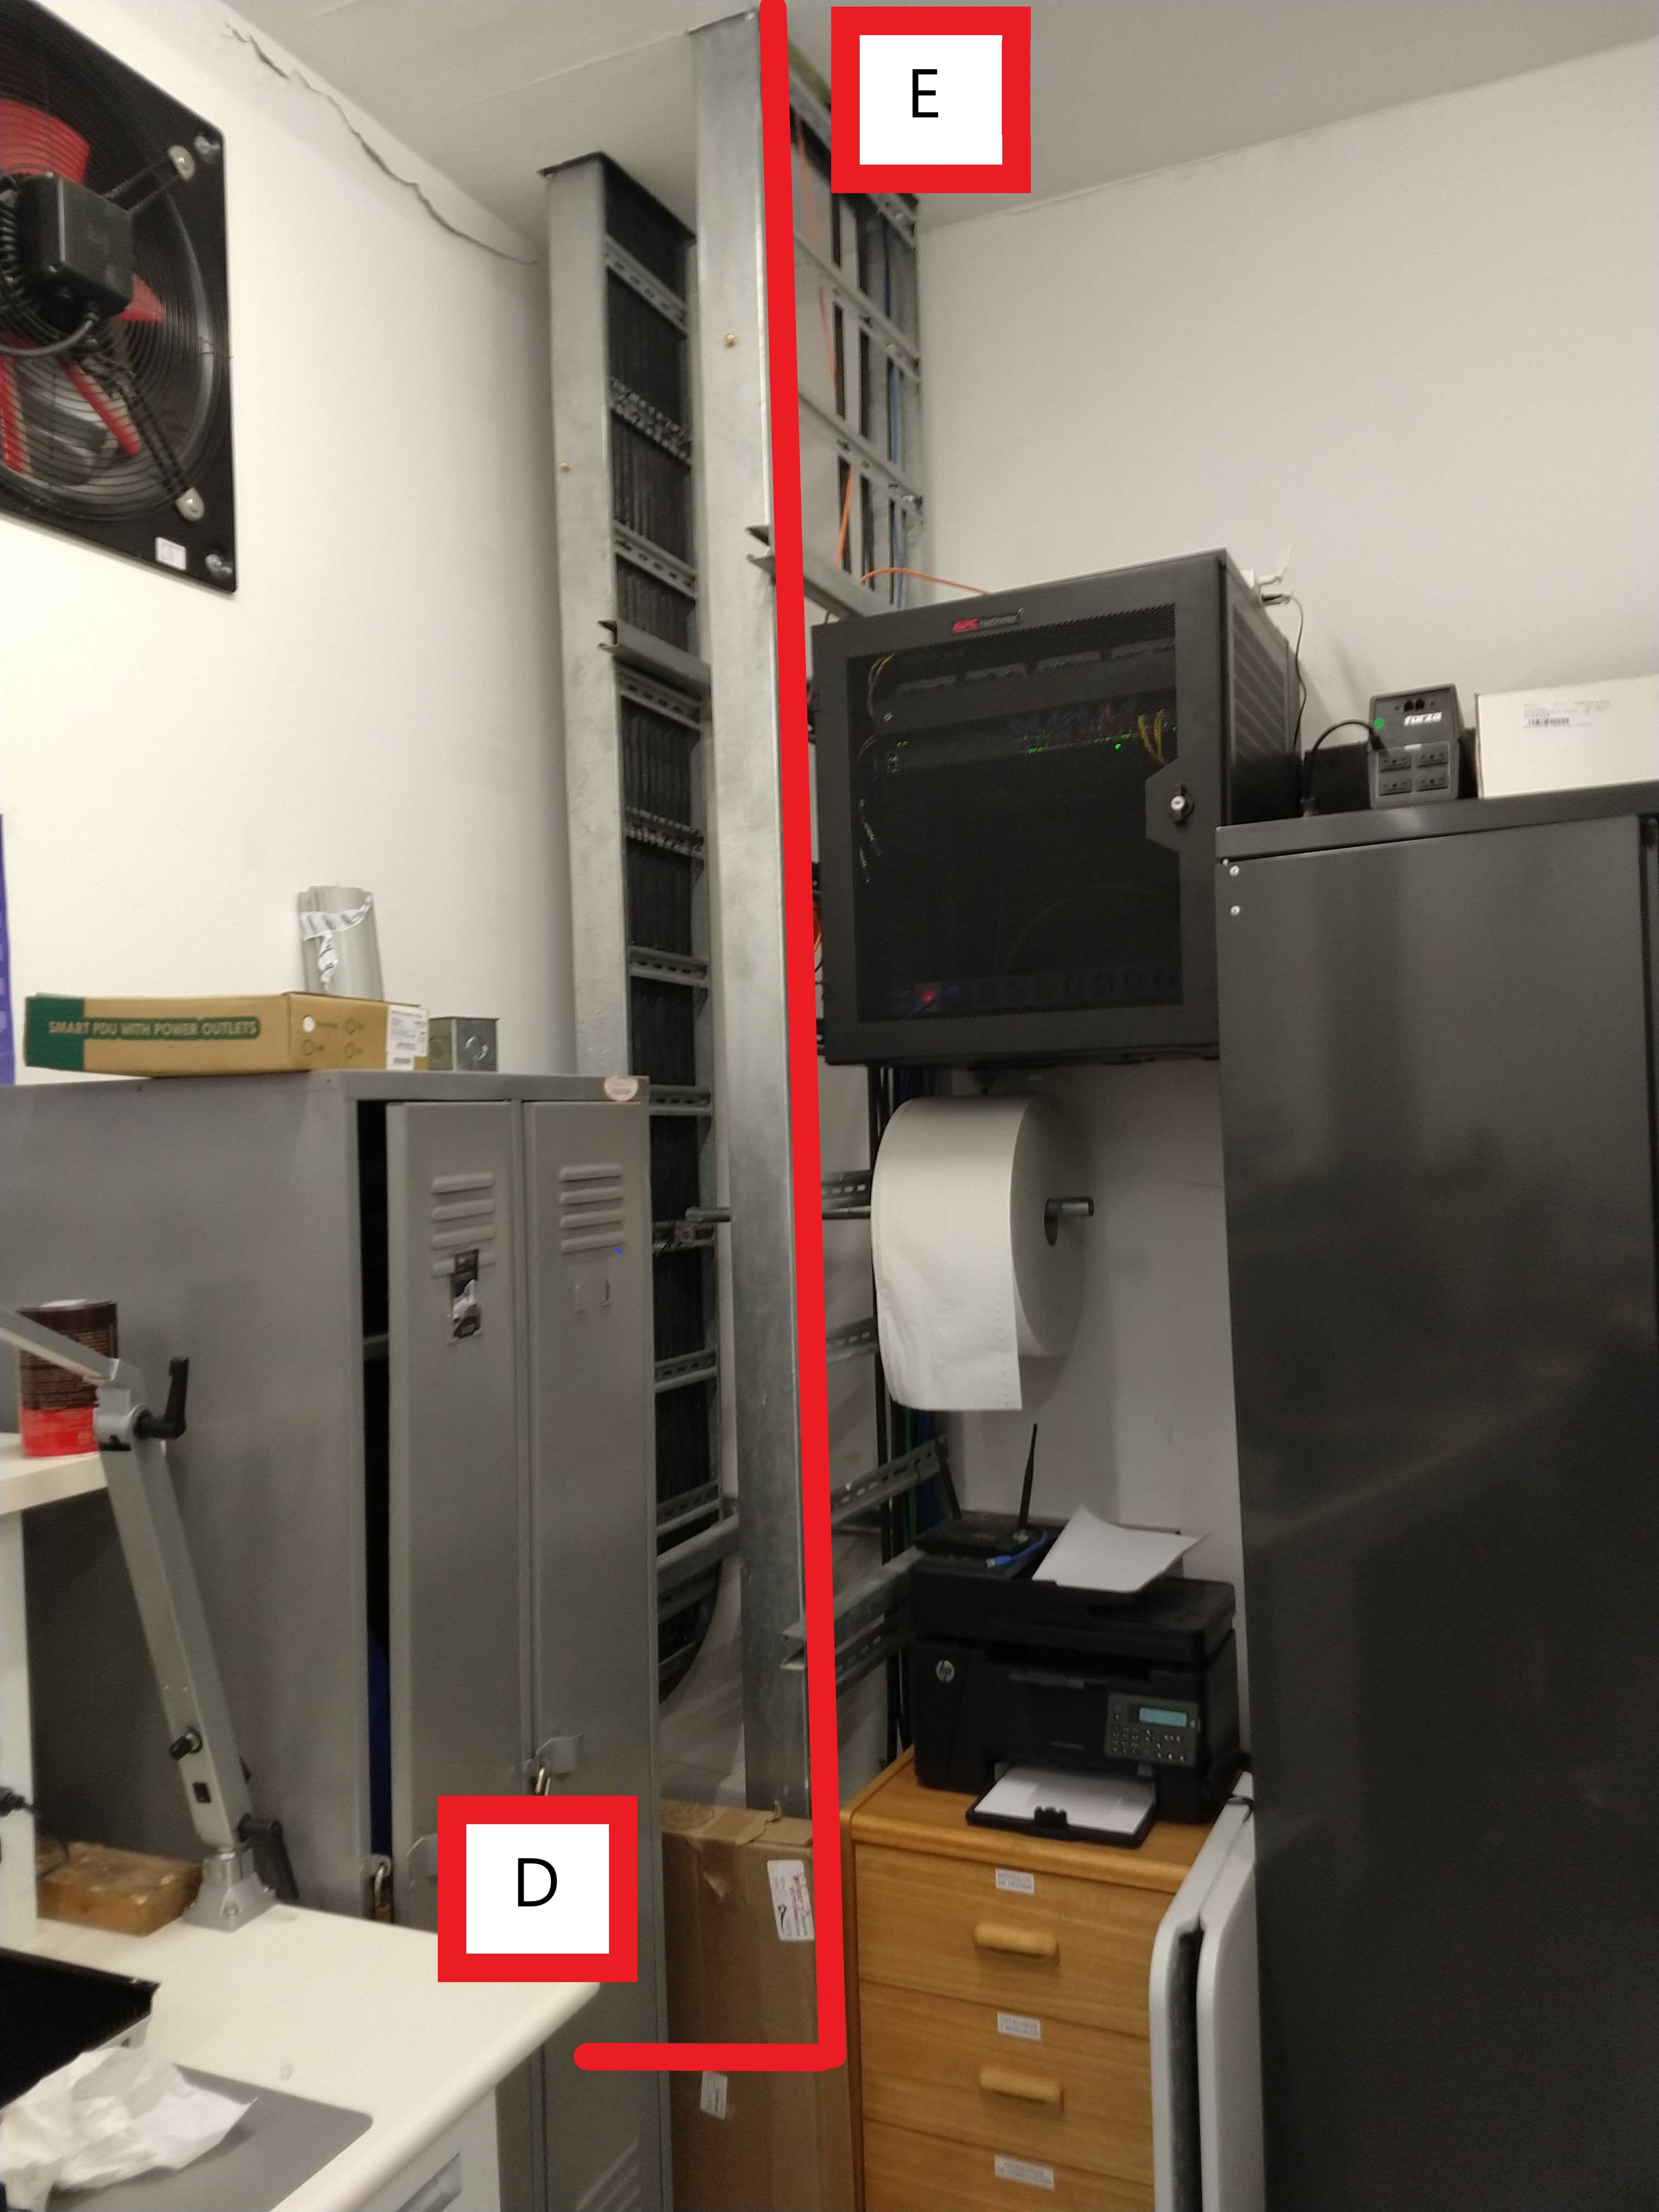
\includegraphics[width=6cm]{images/17.jpg}
\end{figure}

From here the cable goes inside the electronics laboratory room located on the fifth floor and follows the cable tray path to point E.

\begin{figure}
  \centering
  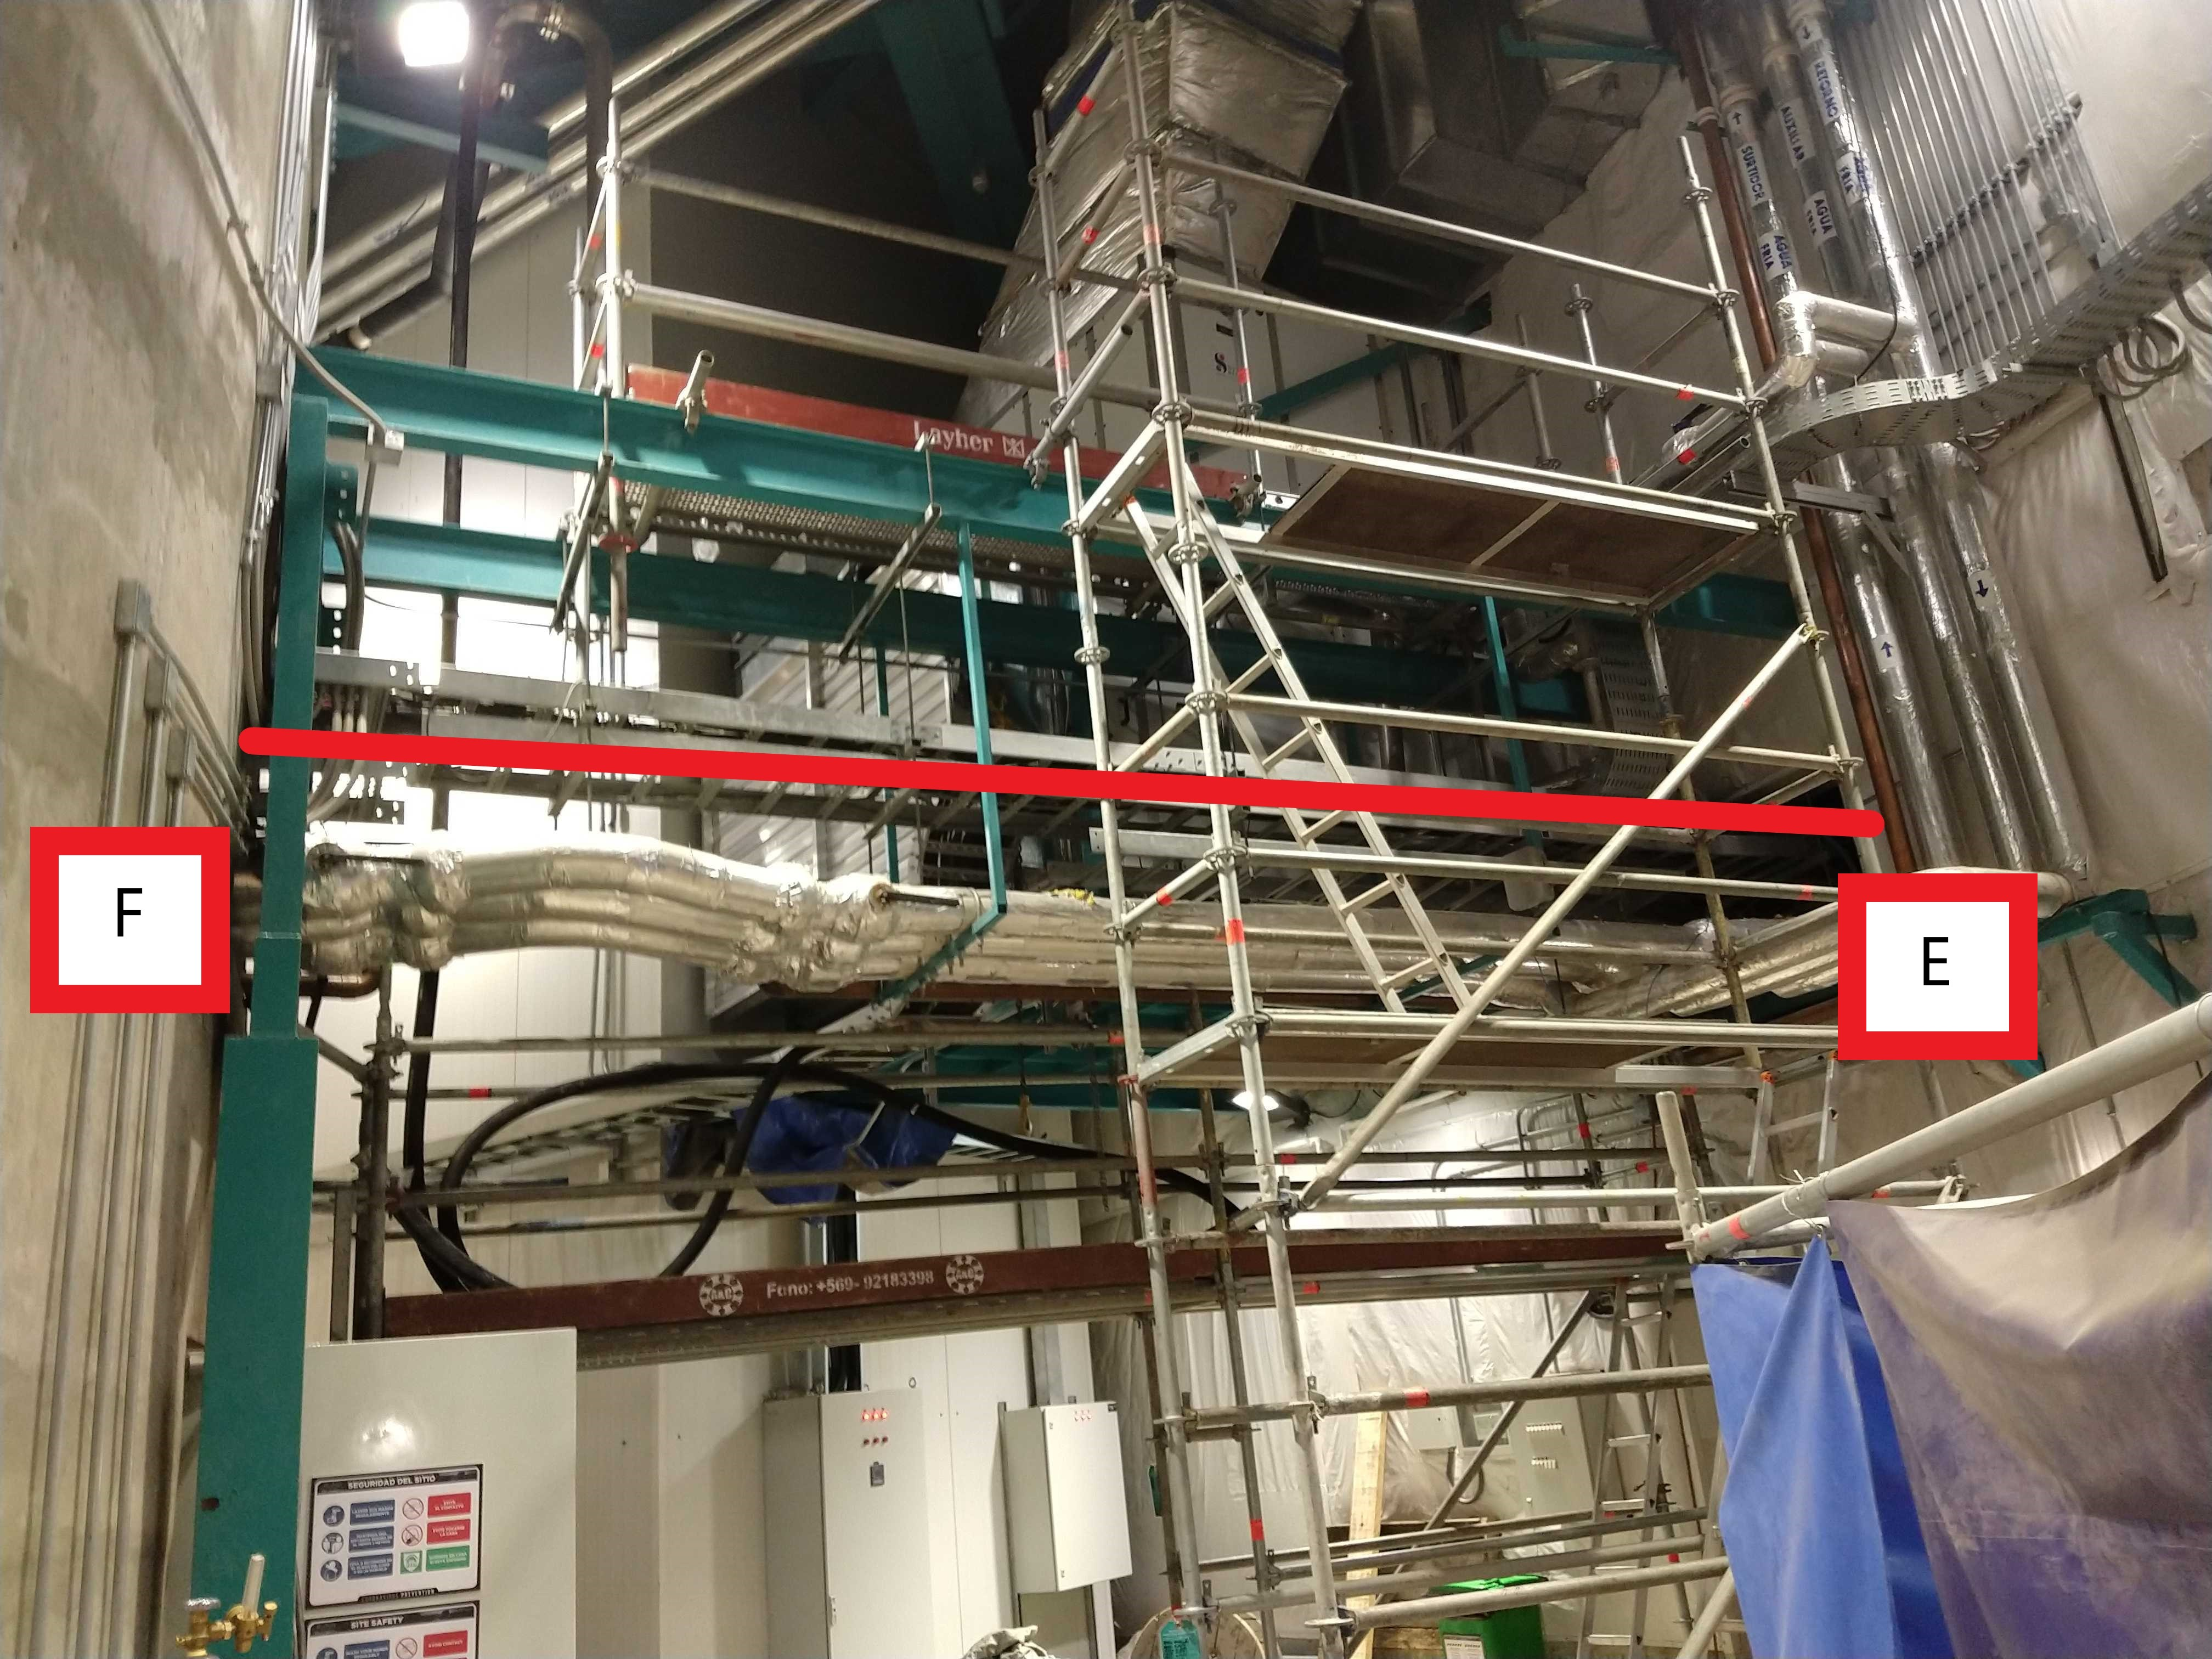
\includegraphics[width=10cm]{images/18.jpg}
\end{figure}

The cable then runs in between the ceiling of the fifth floor and connects to the pier on point F of that same floor.

\begin{figure}
  \centering
  \begin{subfigure}{0.48\textwidth}
    \centering
    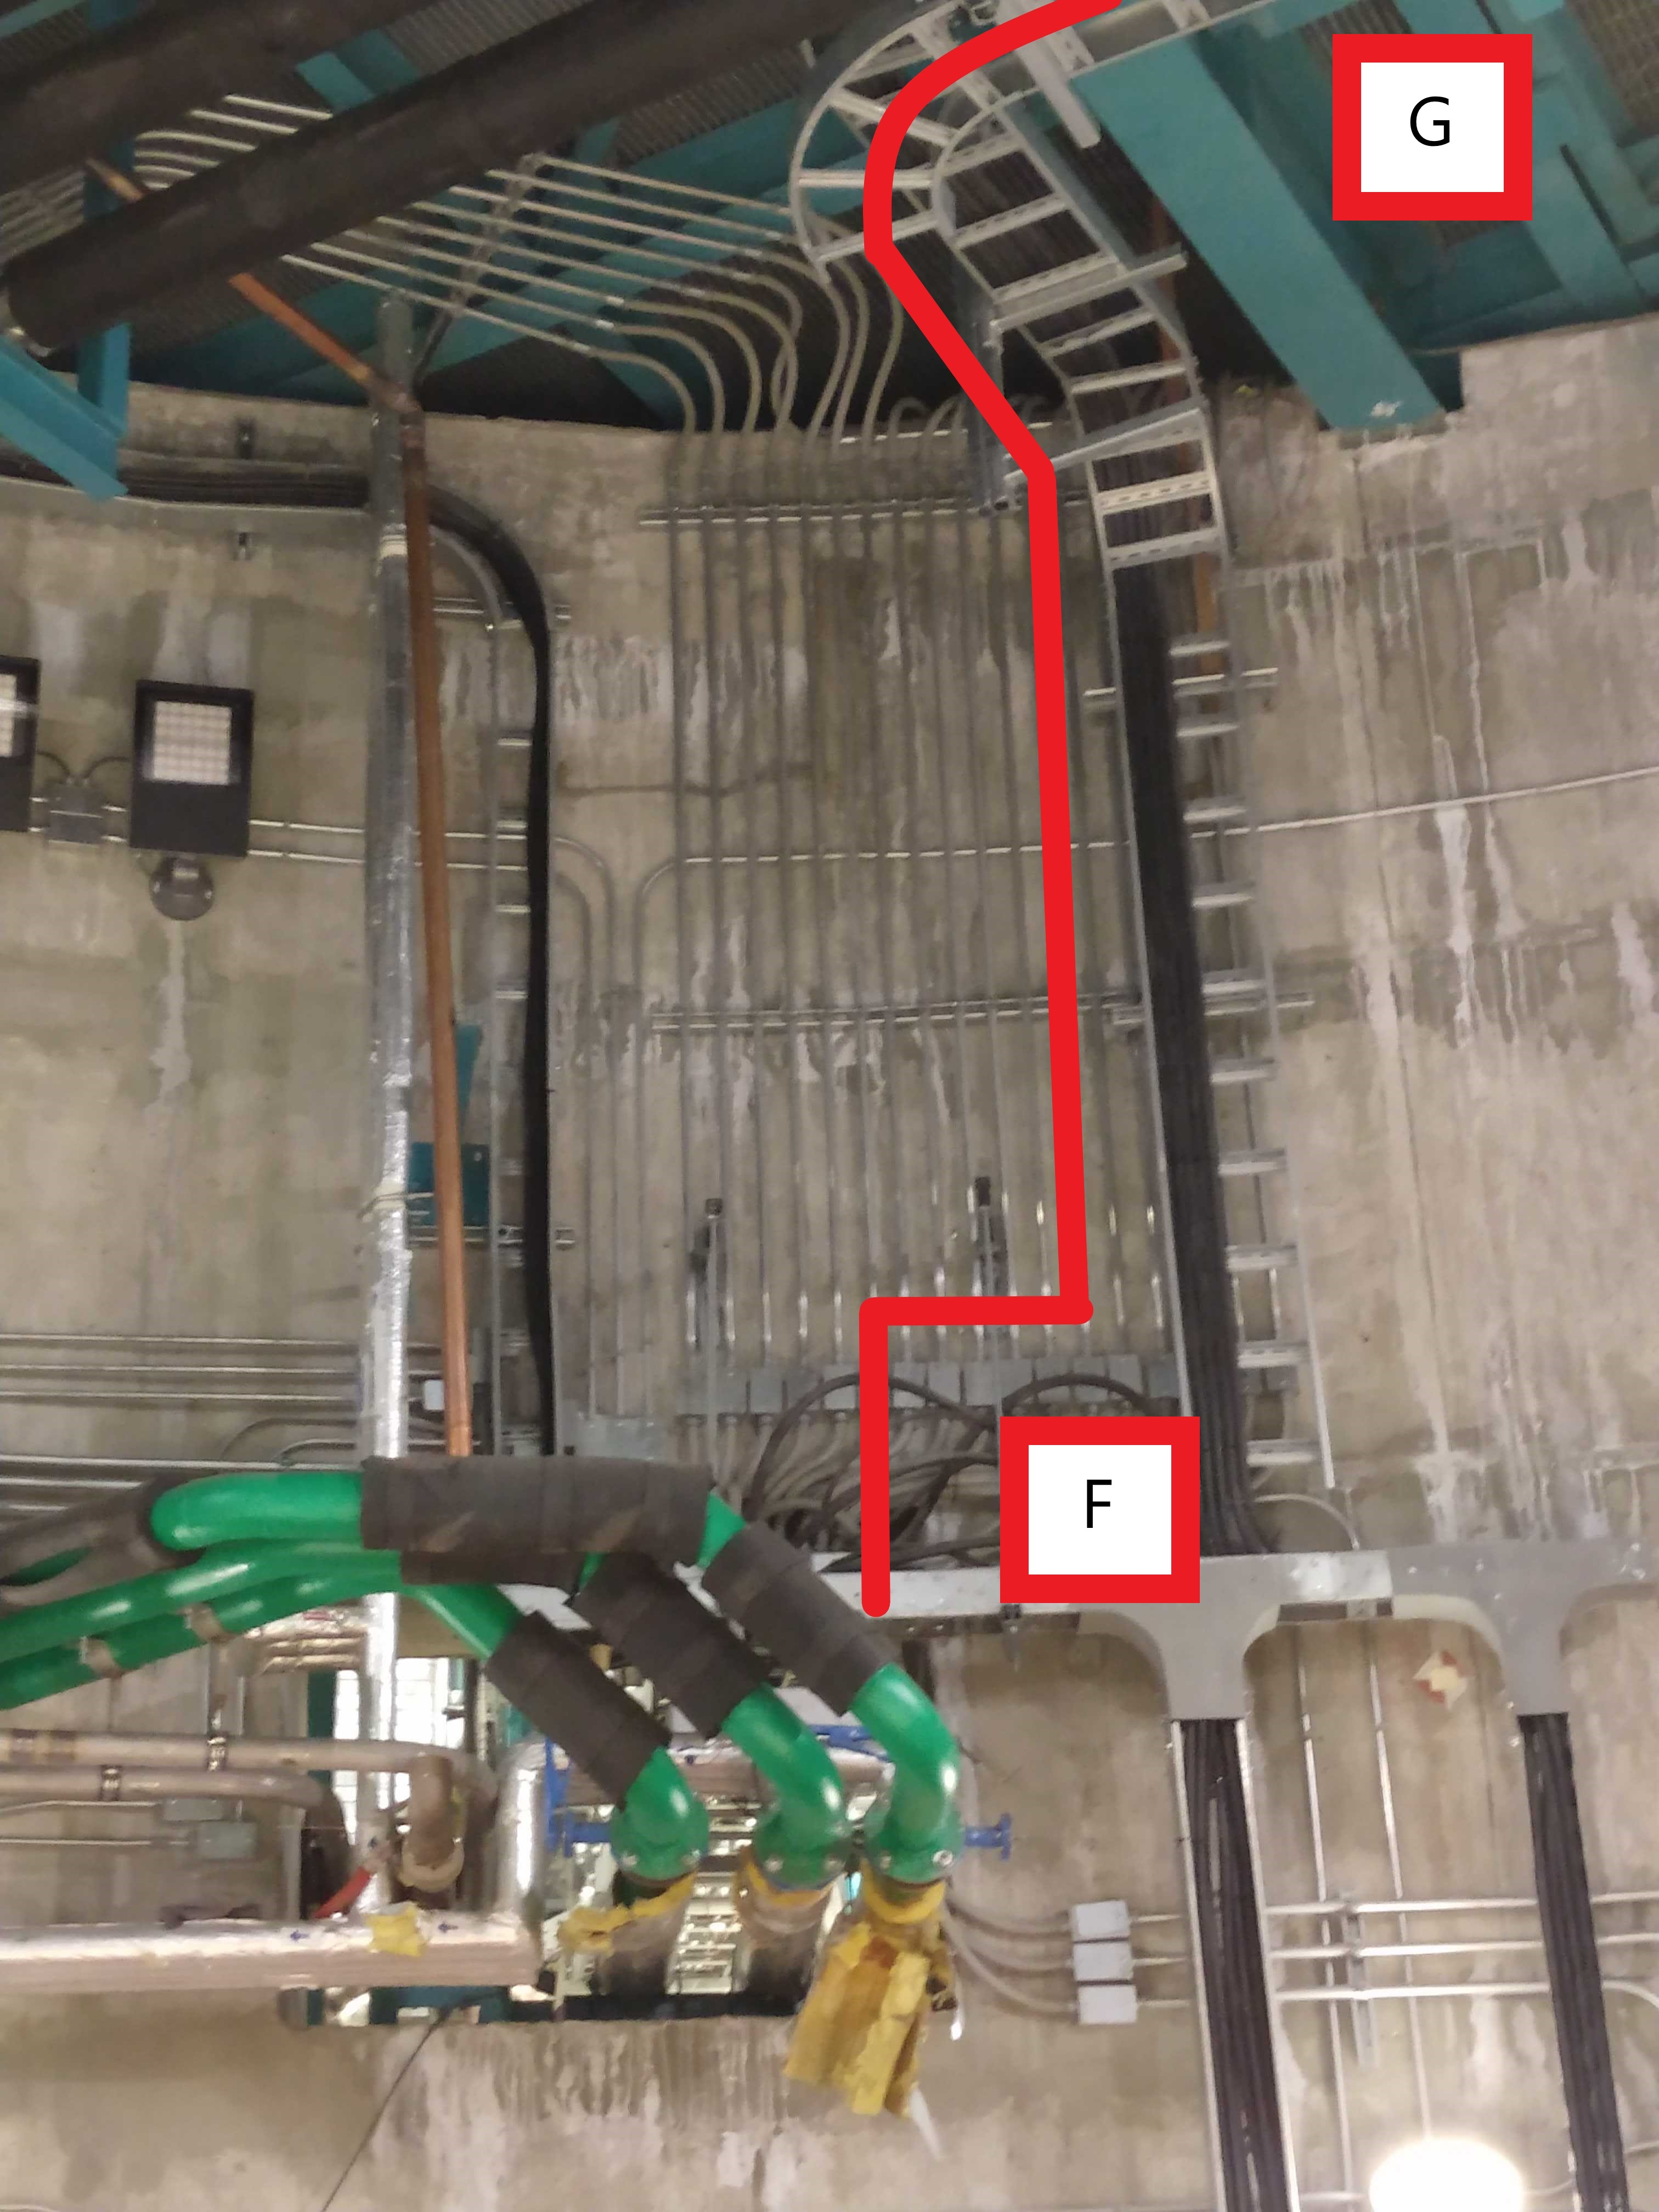
\includegraphics[width=\textwidth]{images/19.jpg}
  \end{subfigure}
  \hfill
  \begin{subfigure}{0.48\textwidth}
    \centering
    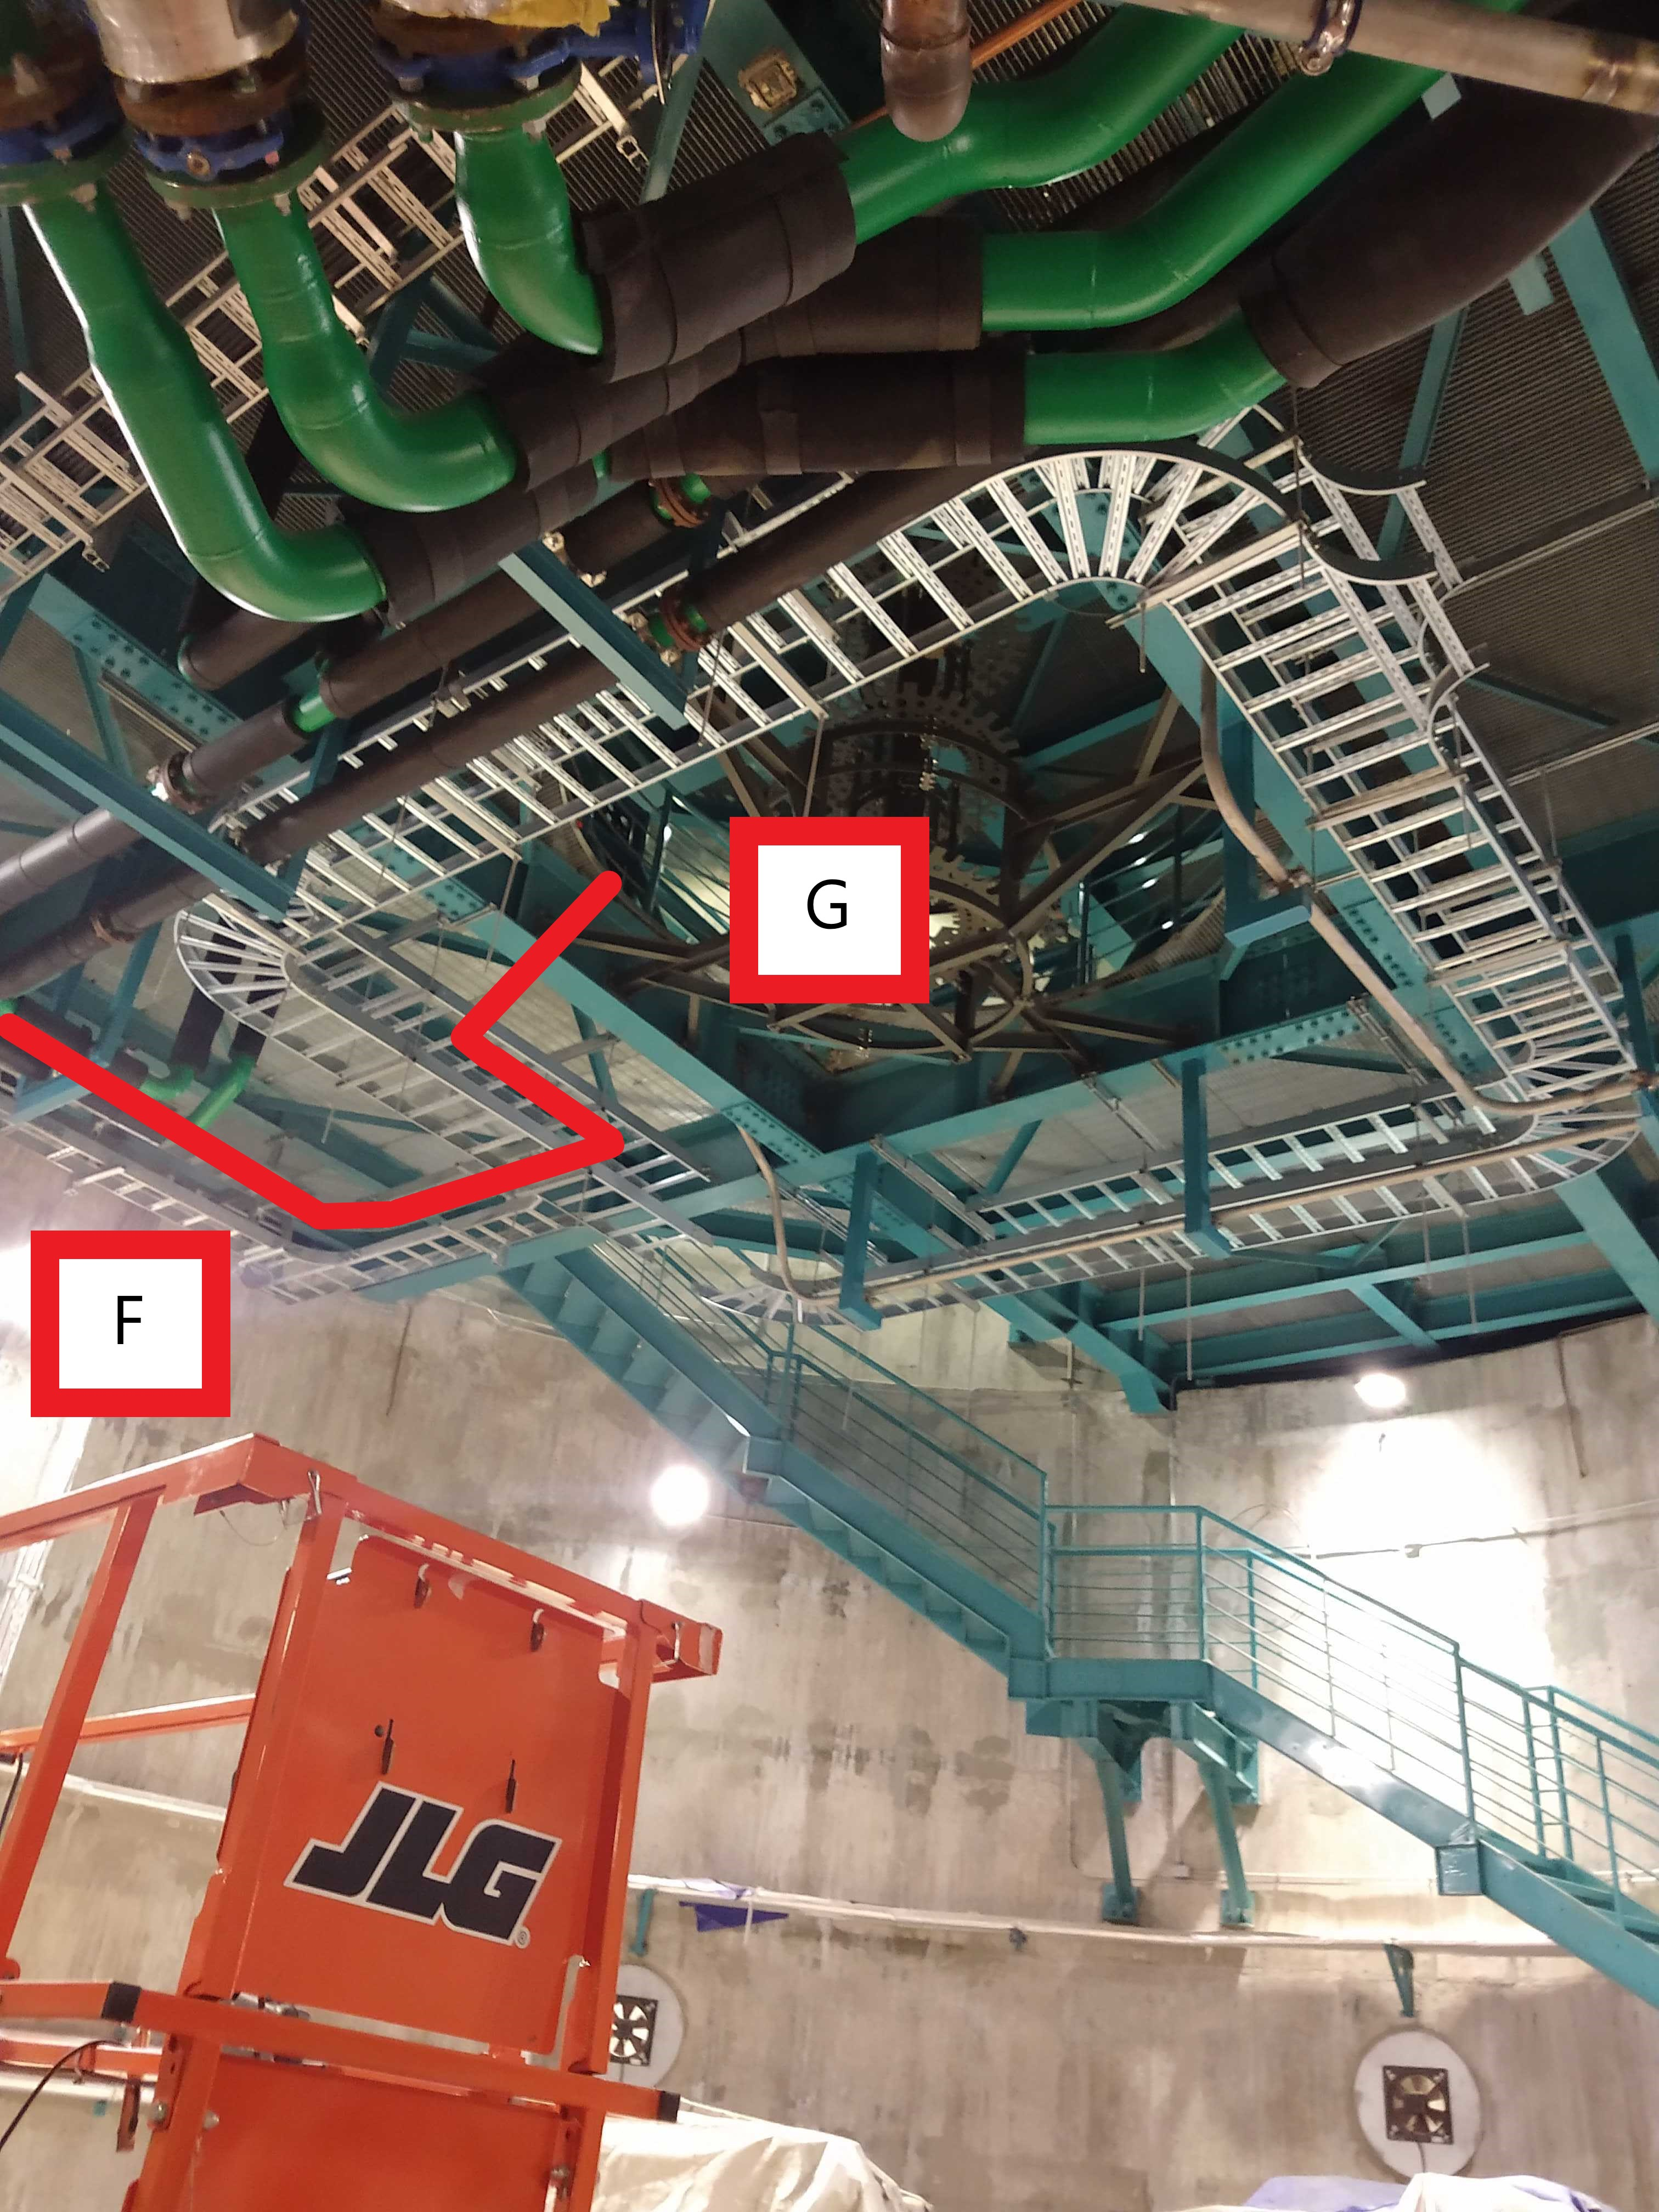
\includegraphics[width=\textwidth]{images/20.jpg}
  \end{subfigure}
\end{figure}
  
\newpage 

  The cable is then finally routed inside the pier from position F in a specifically built cable tray extending to point G.

\begin{figure}
  \centering
  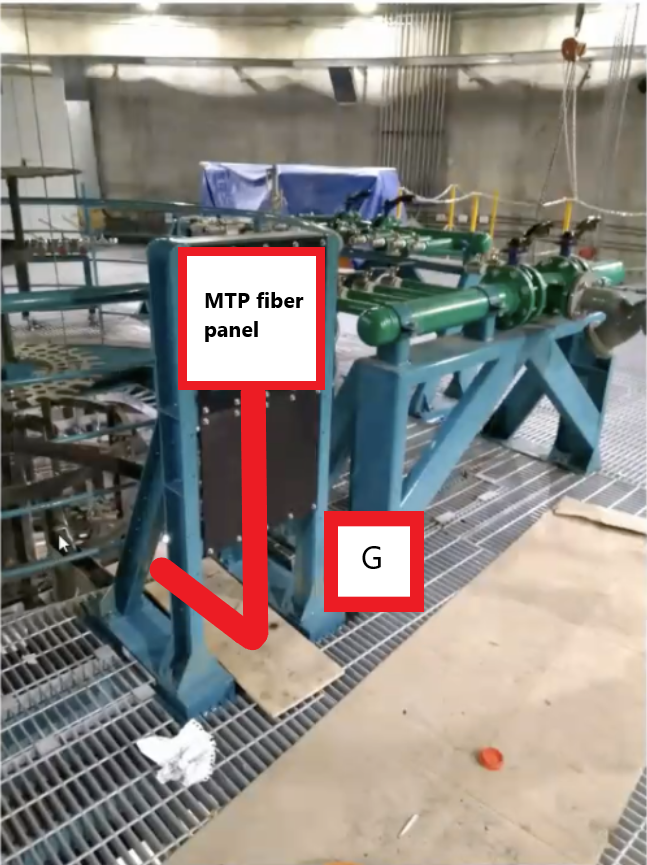
\includegraphics[width=10cm]{images/21.png}
  \caption*{The cable ends in position G on a support mechanism installed on the sixth floor where a connection terminal will be located.}
\end{figure}

\newpage

\subsection{General view of the fiber optic cable disconnect locations}

\begin{figure}
  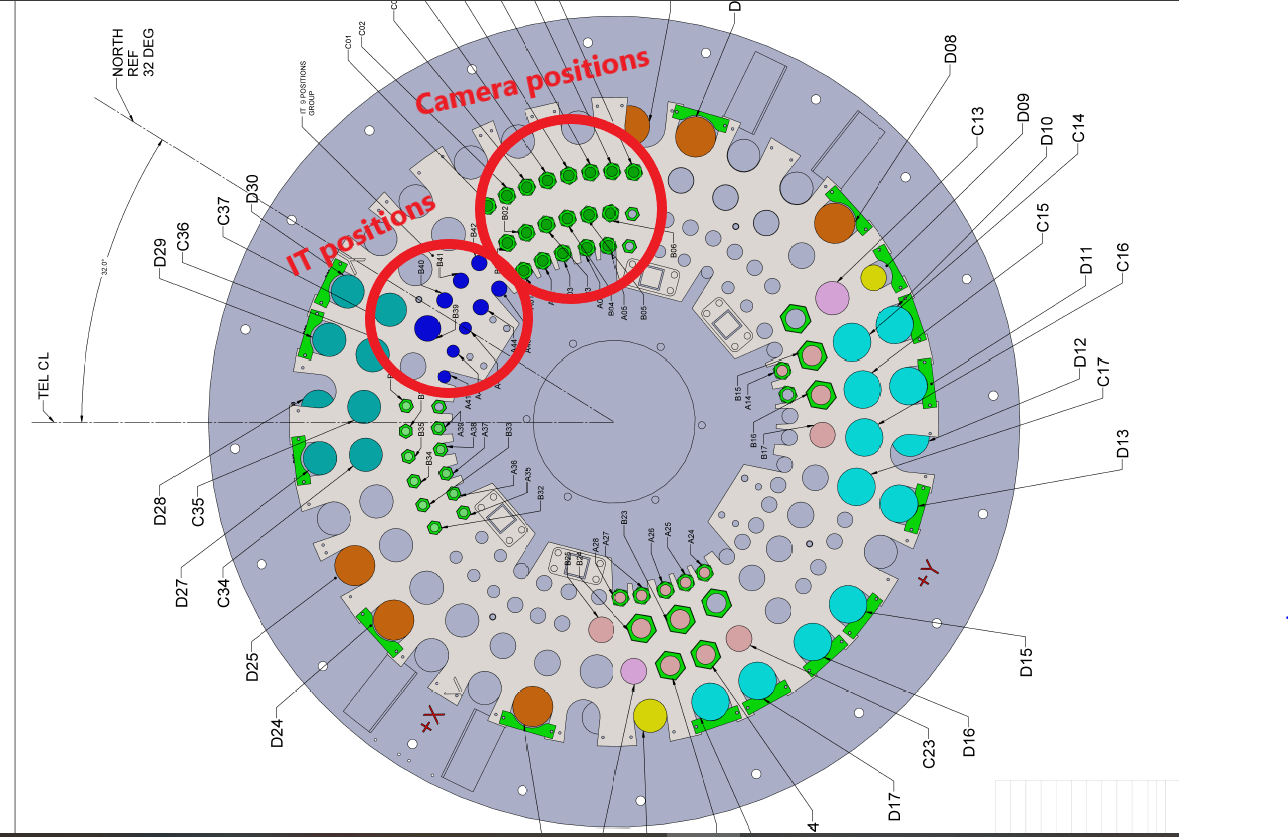
\includegraphics[width=\textwidth]{images/22.png}
\end{figure}

\newpage

\section{Deployment Plan}

  To carry Our deployment plan will begin with the installation of a test fiber to get an exact measurement of the path of the MTP/MPO fiber that will be installed in the future, this cable will extend from point E to D using the image above as reference in bullet 4.2 of the documentation. The document Network Infrastructure Low-Level \footnote[1]{https://confluence.lsstcorp.org/display/IT/Network+Infrastructure+Low-Level+Design+LLD} shows a measurement carried out by a computerized program with an approximate measurement of the length of the cable that is going to be installed. Since this is a custom-built cable we need to know the exact measurements of this cable before pushing out an order to the manufacturer, this is the reason why we are installing this test fiber to get the exact measurement we need.

  The installation of this test cable will require the help of a group of 4 people and work will carry out throughout 3 days taking into account 2 days to install the cable and 1 day to remove it, as of right now we are requesting permission to begin this activity. Once the measurements are taken, we can finally proceed to place an order with the manufacturer for the 13 MTP/MPO cables and an additional 3 more cables as spare. As stated in the document above, this whole process can take up to 2 months before we have the cables on our hands in Chile for use at the summit. Once at the summit, IT will proceed to install the final cables one at a time throughout 3 months approximately.

\newpage

\subsection{Deployment Conclusions and Considerations}

\begin{itemize}
    \item We need at least 3 days to install and uninstall the test cable and to obtain a definitive measurement of the route.
    \item Wait around 2 months for the cables to be delivered and have them at the summit.
    \item All cable installation work must be coordinated one week in advance.
    \item Consider at least 4 people to install the MTP / MPO cables in the future.
    \item It will take about 32 days of actual work to install the 16 MTP / MPO cables, working at least 3 times a week.
    \item When installing the cables, we have to pay close attention to the gender of the connector of the cable.
    \item The female connector will be located in the computer room and the male connector will be on the sixth floor.
\end{itemize}

\newpage